\chapter{Quantification of Spatial Self-Shielding Effects}
\label{chap:quantify}


%%%%%%%%%%%%%%%%%%%%%%%%%%%%%%%%%%%%%%%%%%%%%%%%%%%%%%%%%%%%%%%%%%%%%%%%%%%%%%%
\section{Overview}
\label{sec:chap8-overview}

-Can this section be merged with the following one???

first paragraph: motivate, chapter objectives
-generate MGXS for large heterogeneous geometries
-connect with preceding chapter
-objective for chapter:
  -quantify error ``gap'' resolved when spatial self-shielding is ``fully'' accounted for
  -we are using the reference solution computed for each benchmark in Chap.~\ref{chap:benchmarks}

second paragraph: outline chapter
-Sec.~\ref{sec:chap8-pinwise-space-homogenize}
-Sec.~\ref{sec:chap8-moc-params}
-Sec.~\ref{sec:chap8-mg-results}
-Sec.~\ref{sec:chap8-mgxs-converge}


%%%%%%%%%%%%%%%%%%%%%%%%%%%%%%%%%%%%%%%%%%%%%%%%%%%%%%%%%%%%%%%%%%%%%%%%%%%%%%%
\section{Pin-wise Spatial Homogenization Schemes}
\label{sec:chap8-pinwise-space-homogenize}

first paragraph: intro paragraph?
-motivation is to explore impact of using proper spatial self-shielding on fuel pins ONLY
-used \texttt{openmc.mgxs} module to tally 70-group \ac{MGXS} in each case
  -collapsed to 2-group and 8-group \ac{MGXS} in downstream data processing
-Fig.~\ref{fig:chap8-homogenization-schemes} illustrates the materials and \ac{MGXS}
  -infinite, null and degenerate schemes
-Tab.~\ref{table:chap8-num-materials} - number of unique materials / \ac{MGXS} for each geometry with each scheme

second paragraph: outline
-outline following sections

-1e6 particles / batch, 1000 batches to tally \ac{MGXS} for each benchmark
  -the same parameters used to generate the reference solutions in the preceding chapter

-need summary box for this section
-rethink names for null and degenerate???
-re-color the water, fuel, etc.!!!

\begin{table}[h!]
  \centering
  \caption[Number of multi-group material for each spatial homogenization scheme]{Number of multi-group materials modeled with unique \ac{MGXS} in each heterogeneous benchmark for each spatial homogenization scheme.}
  \small
  \label{table:chap8-num-materials}
  \vspace{6pt}
  \begin{tabular}{l r r r}
  \toprule
  \rowcolor{lightgray}
  & \multicolumn{3}{c}{\cellcolor{lightgray} \bf \# Materials} \\
  \multirow{-2}{*}{\cellcolor{lightgray} \bf Benchmark} &
  {\cellcolor{lightgray} \bf Infinite} &
  {\cellcolor{lightgray} \bf Null} &
  {\cellcolor{lightgray} \bf Degenerate} \\
  \midrule
1.6\% Assm & 8 & 8 & 271 \\
  \midrule
3.1\% Assm & 8 & 8 & 271 \\
  \midrule
3.1\% Assm w/ 20 BPs & 10 & 10 & 273  \\
  \midrule
2$\times$2 Colorset & 11 & 11 & 1065 \\
  \midrule
2$\times$2 Colorset w/ Reflector & 11 & 11 & 1065 \\
  \midrule
\ac{BEAVRS} Full Core & 15 & 15 & 50,961 \\
  \bottomrule
\end{tabular}
\end{table}


\begin{figure}[h!]
\centering
\begin{subfigure}{.5\textwidth}
  \centering
  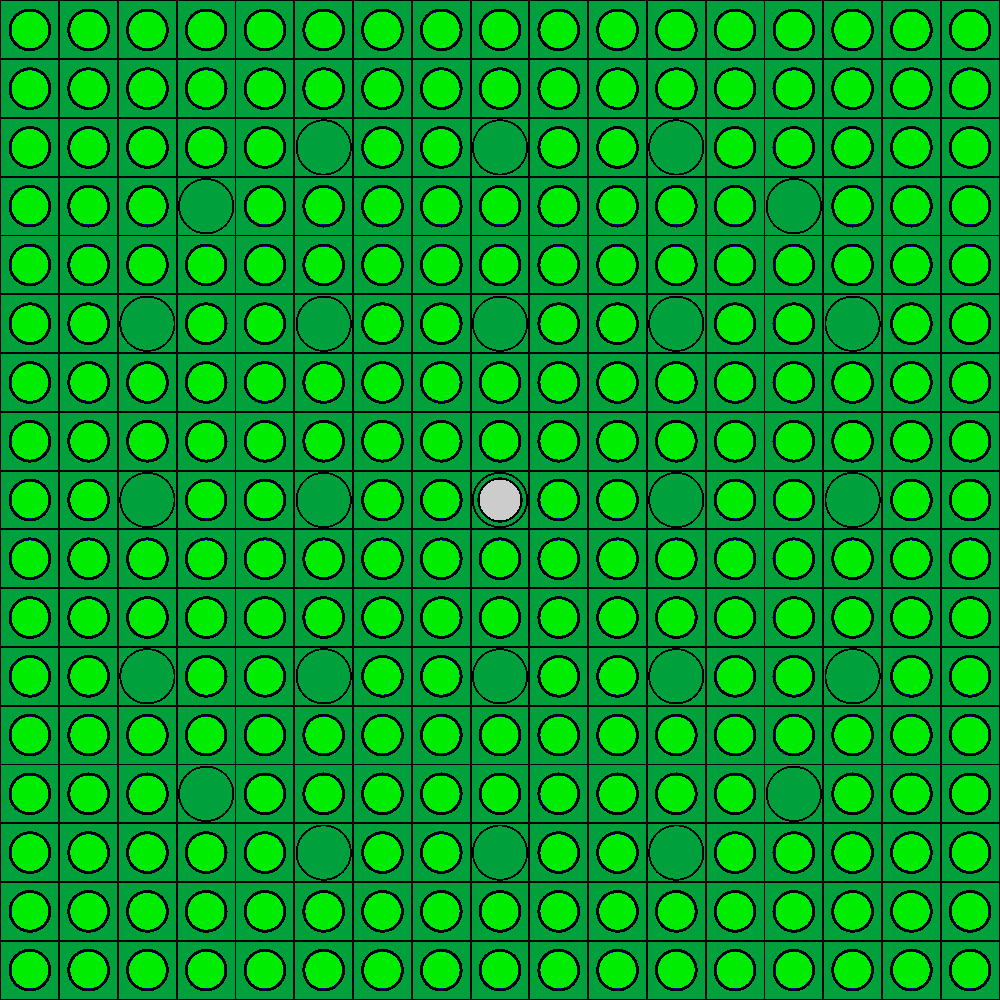
\includegraphics[width=0.8\linewidth]{figures/quantification/homogenization/assm-16-null-materials}
  \caption{}
  \label{fig:chap8-assm-16-null-materials}
\end{subfigure}%
\begin{subfigure}{.5\textwidth}
  \centering
  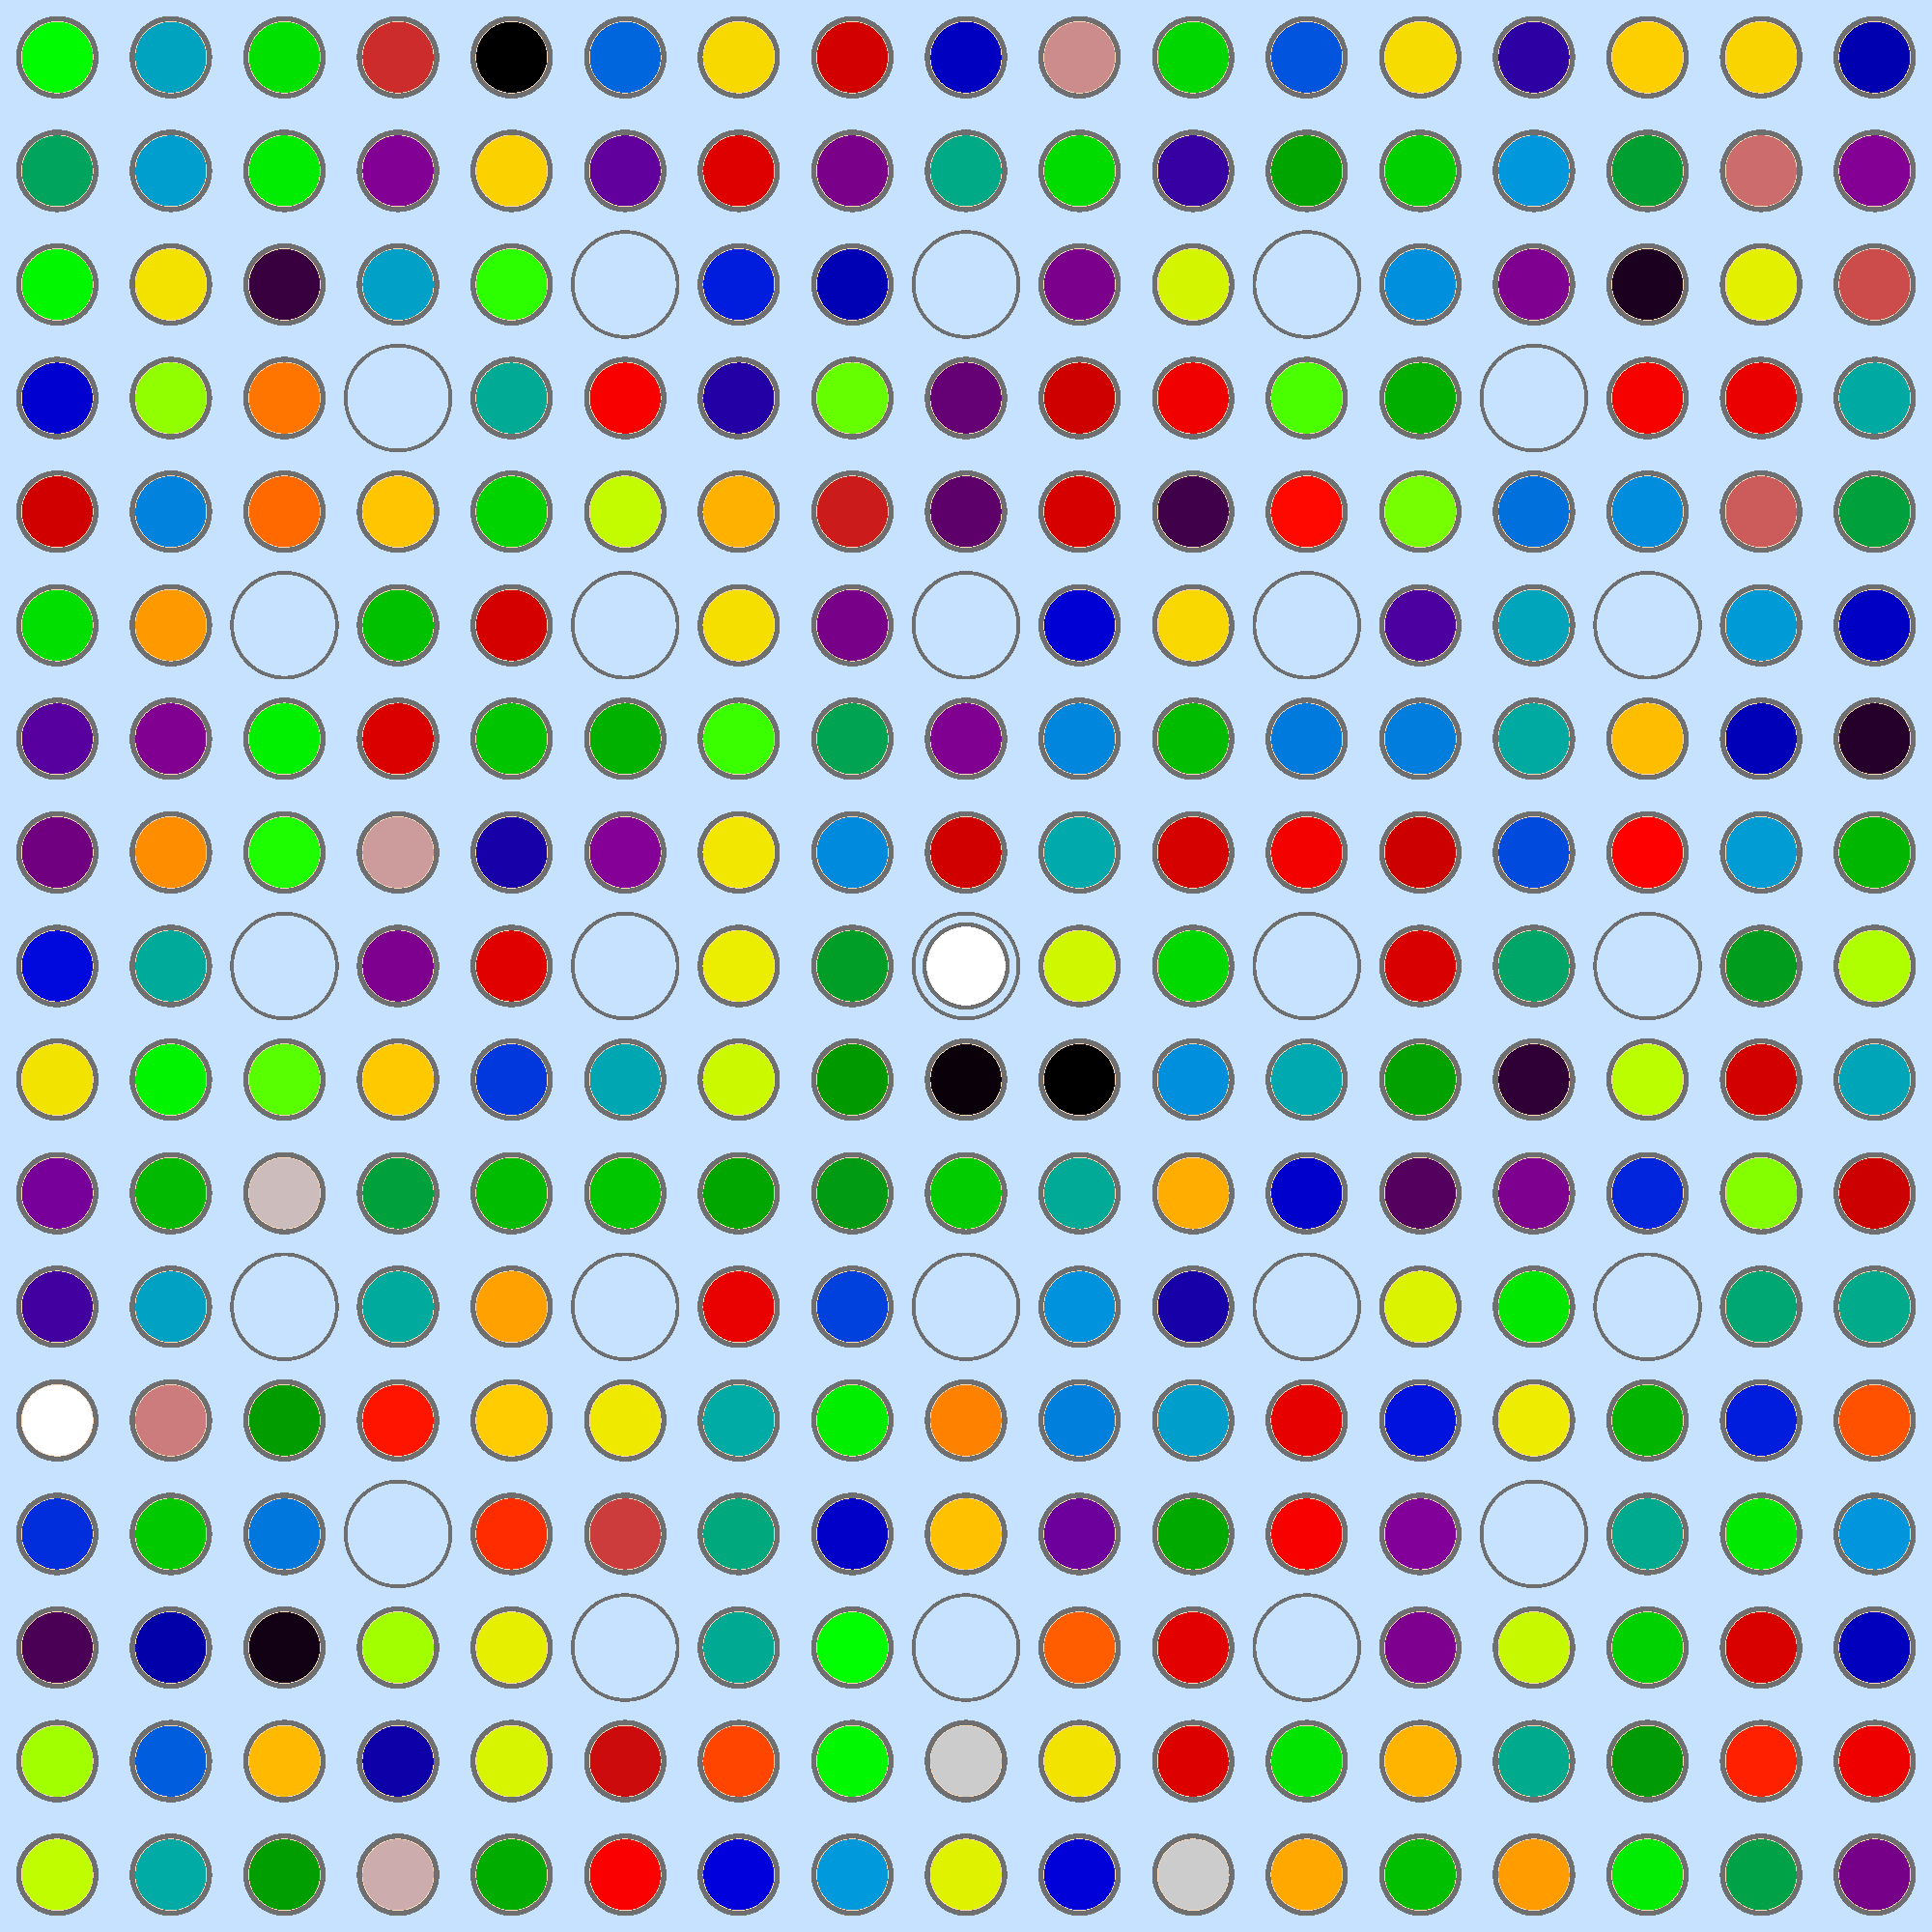
\includegraphics[width=0.8\linewidth]{figures/quantification/homogenization/assm-16-degenerate-materials}
  \caption{}
  \label{fig:chap8-assm-16-degenerate-materials}
\end{subfigure}
\begin{subfigure}{.5\textwidth}
  \centering
  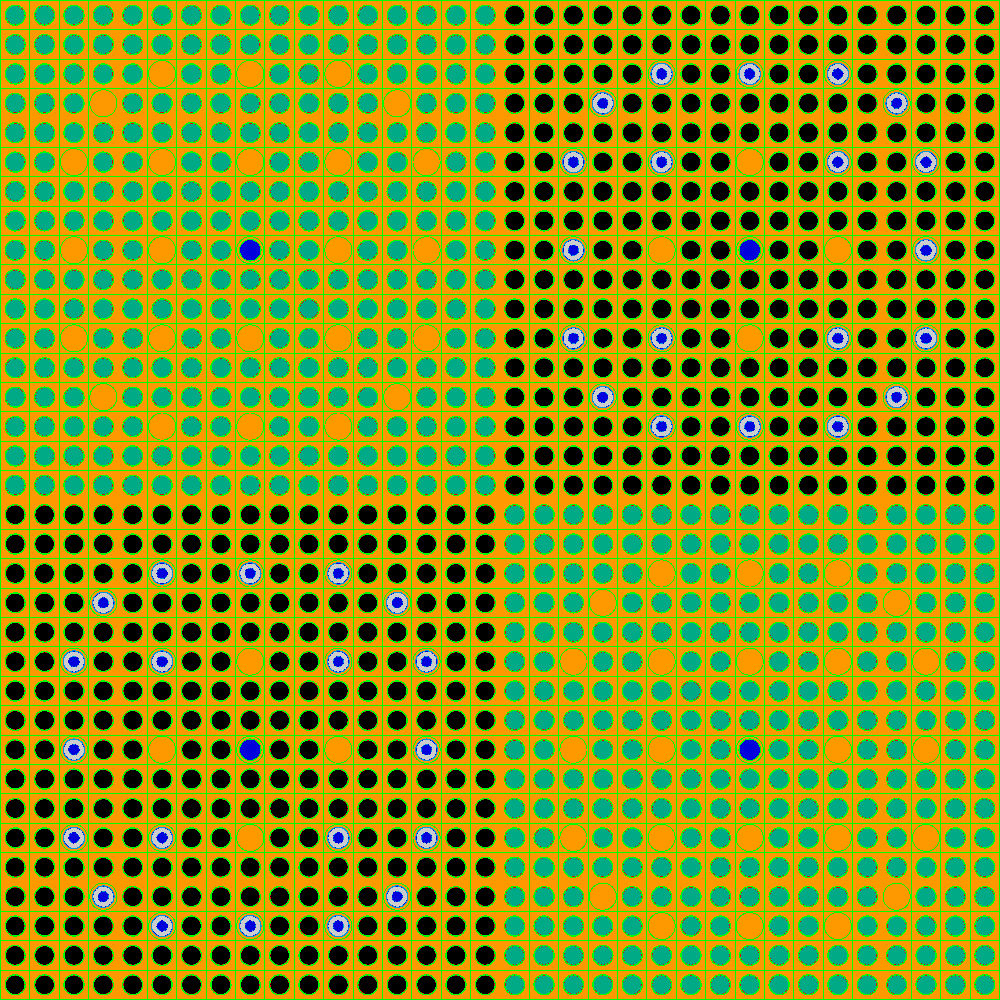
\includegraphics[width=0.8\linewidth]{figures/quantification/homogenization/2x2-null-materials}
  \caption{}
  \label{fig:chap8-2x2-null-materials}
\end{subfigure}%
\begin{subfigure}{.5\textwidth}
  \centering
  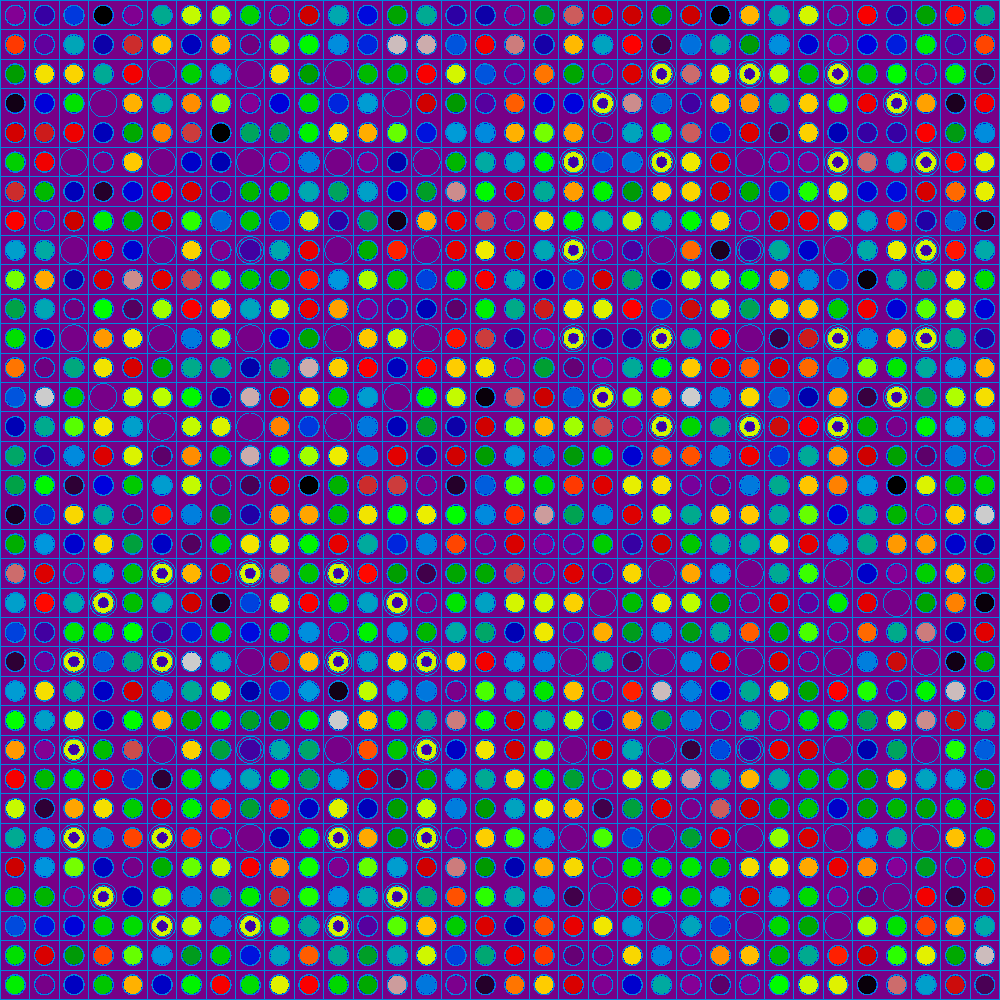
\includegraphics[width=0.8\linewidth]{figures/quantification/homogenization/2x2-degenerate-materials}
  \caption{}
  \label{fig:chap8-2x2-degenerate-materials}
\end{subfigure}
\begin{subfigure}{.5\textwidth}
  \centering
  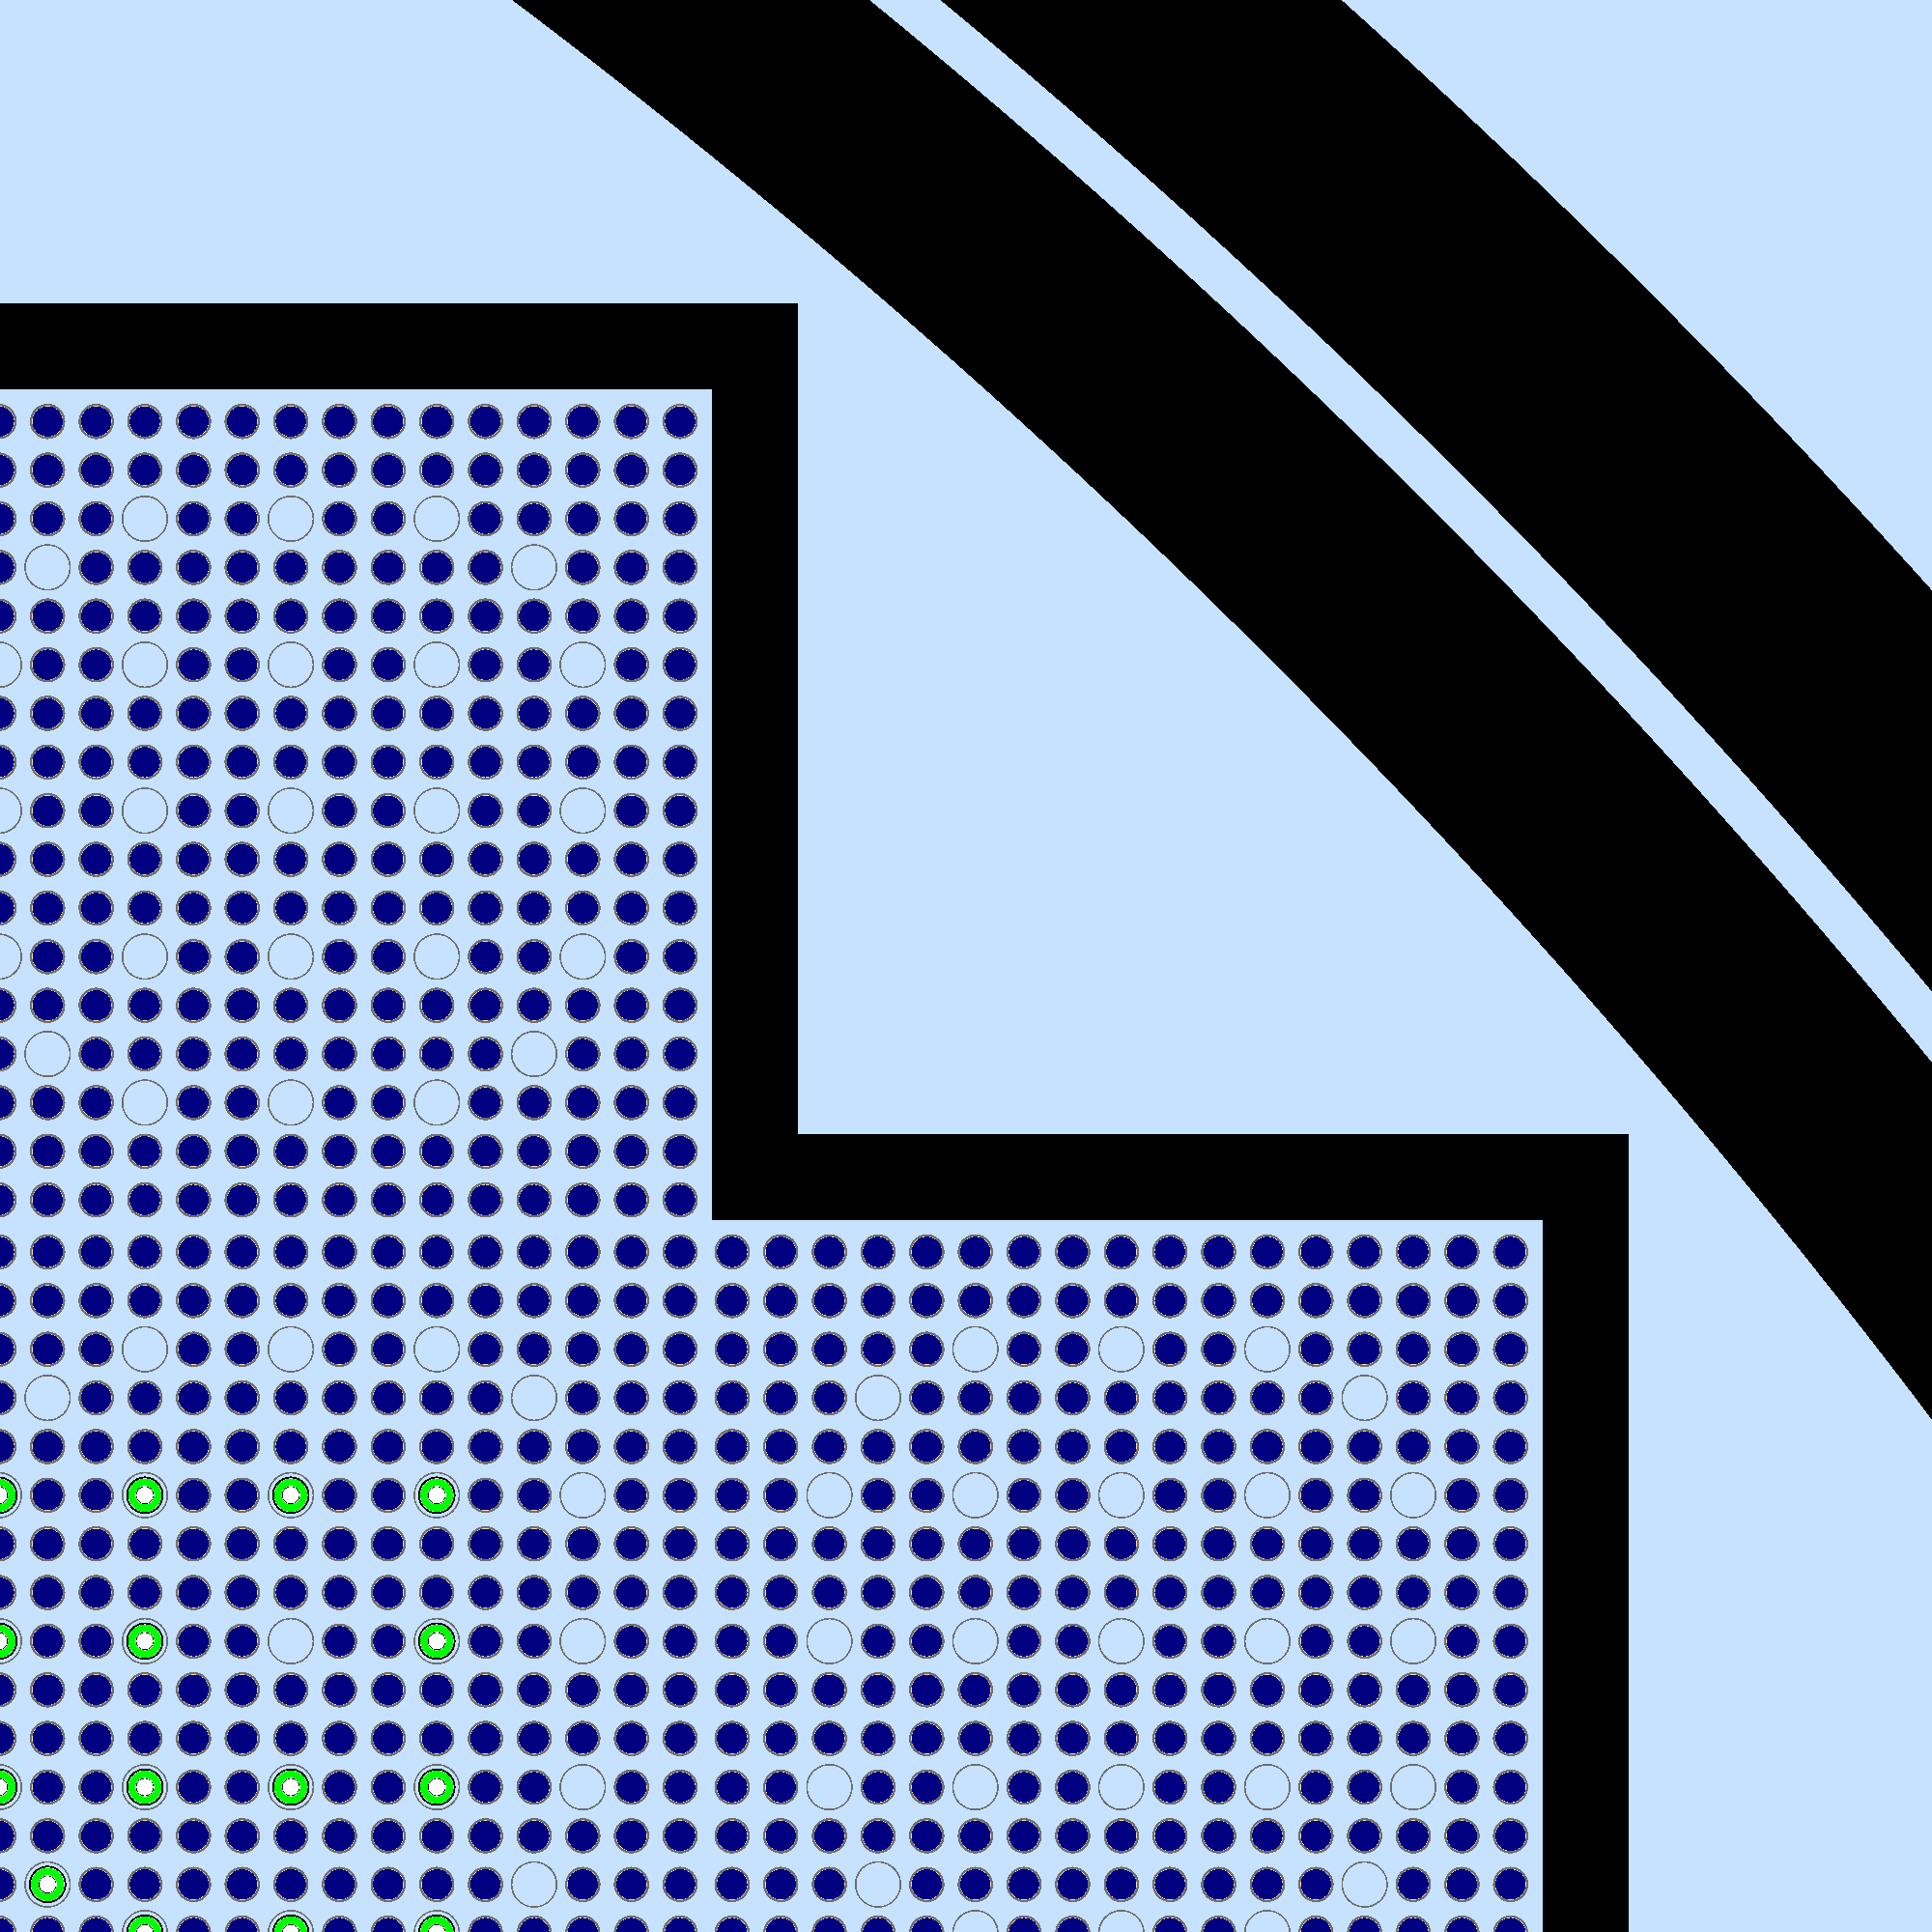
\includegraphics[width=0.8\linewidth]{figures/quantification/homogenization/full-core-null-materials}
  \caption{}
  \label{fig:chap8-full-core-null-materials}
\end{subfigure}%
\begin{subfigure}{.5\textwidth}
  \centering
  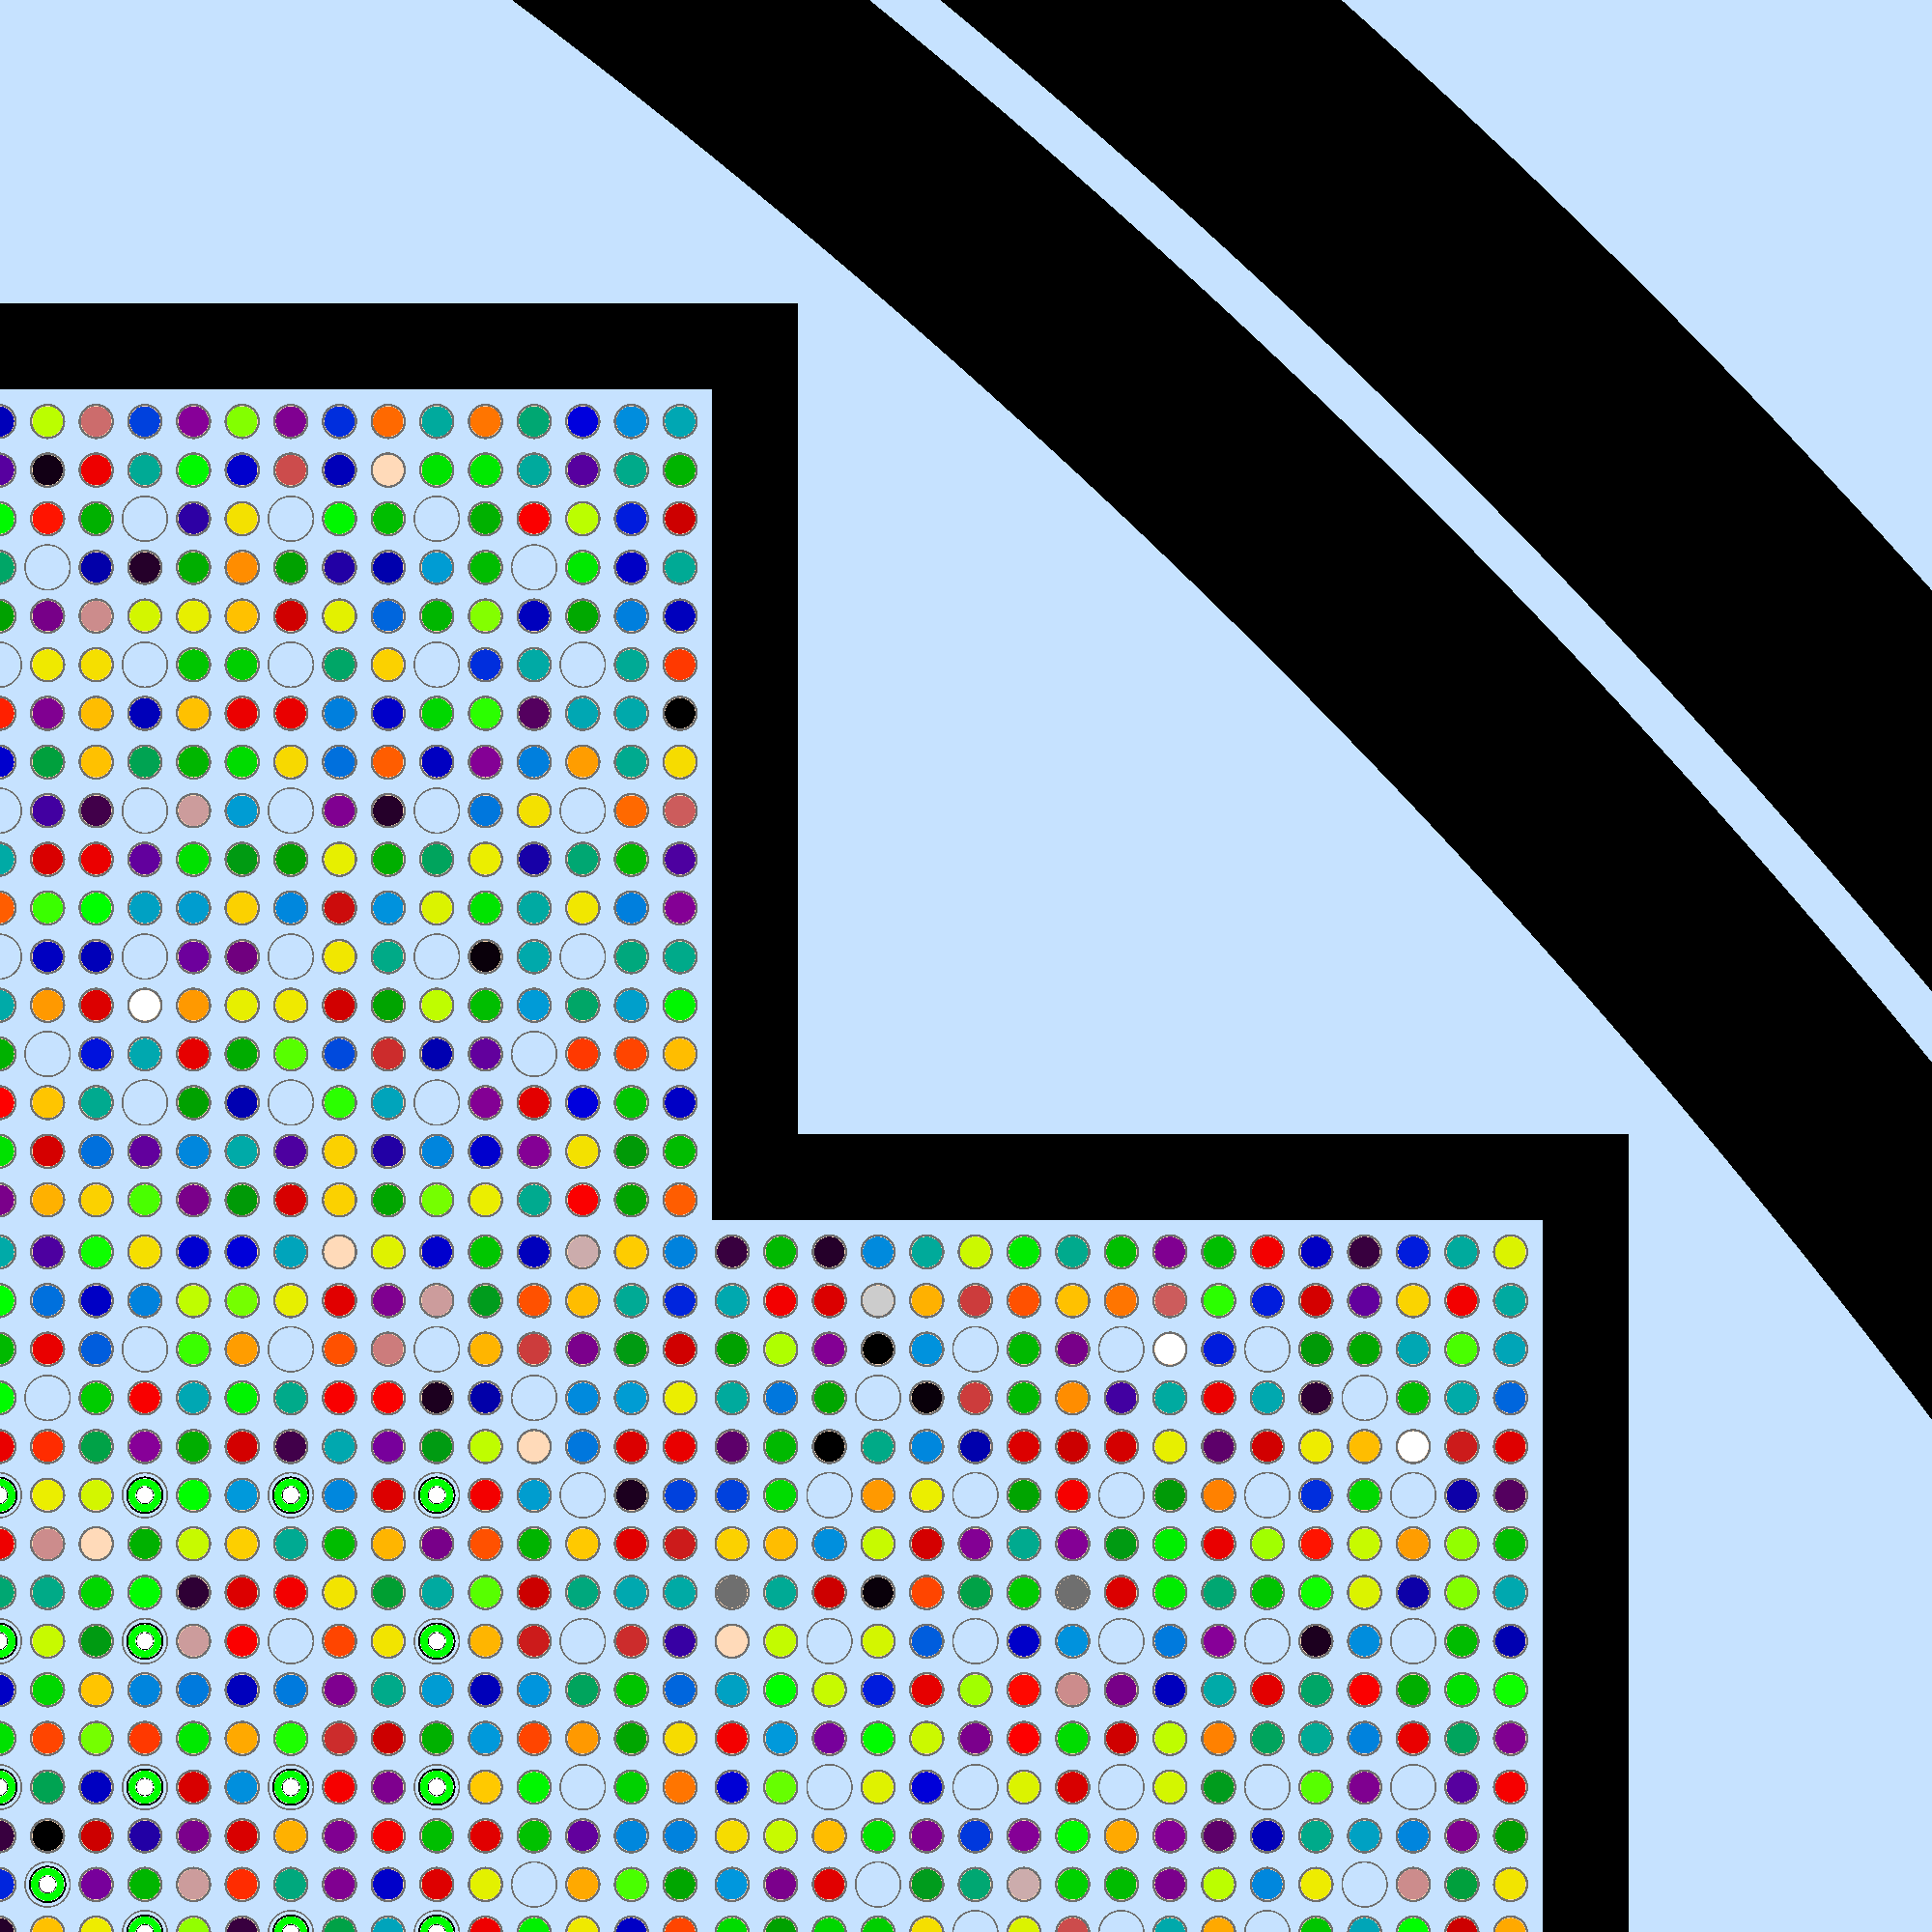
\includegraphics[width=0.8\linewidth]{figures/quantification/homogenization/full-core-degenerate-materials}
  \caption{}
  \label{fig:chap8-full-core-degenerate-materials}
\end{subfigure}
\caption[Depiction of infinite, null and degenerate spatial homogenization schemes]{OpenMOC materials for a single fuel assembly, a 2$\times$ colorset and the 2D full core \ac{BEAVRS} model. The materials for the infinite and null schemes are depicted in (a), (c) and (e), and for the degenerate scheme in (b), (d) and (f), respectively. Each uniquely colored material represents a unique set of self-shielded \ac{MGXS}.}
\label{fig:chap8-homogenization-schemes}
\end{figure}

%%%%%%%%%%%%%%%%%%%%%%%%%%%%%%%%%%%%%%
\subsection{Infinite Lattice Homogenization}
\label{subsec:chap8-infinite}

first paragraph: infinite scheme
-use OpenMC cell tallies for \ac{MGXS} in two different geometries
-model each type of fuel pin (each enrichment) and compute \ac{MGXS} in an infinite lattice
-compute \ac{MGXS} for other pin types -- \acp{CRGT}, \acp{BP}, instr tubes -- in original lattice
-\ac{MGXS} computed for each single (infinitely repeated) fuel pin cell 
-each instance of a unique fuel pin type (e.g, enrichment) gets a single type of \ac{MGXS}
-foonote: unable to run infinite pin cell calculations for non-fissile pin cells (CRGTs, BPs, instr tubes) since it's not a criticality calculation
-neglects (averages over) the different spatial self-shielding effects experienced in each fuel pin

%%%%%%%%%%%%%%%%%%%%%%%%%%%%%%%%%%%%%%
\subsection{Null Homogenization}
\label{subsec:chap8-null}

first paragraph: null scheme
-used OpenMC cell tallies in the same heterogeneous geometry we wish to model with OpenMC
-each instance of a unique fuel pin type (e.g, enrichment) gets a single type of \ac{MGXS}
-the spectrum used to collapse / homogenize \ac{MGXS} is more appropriate than that used for infinite
-neglects (averages over) the different spatial self-shielding effects experienced in each fuel pin

%%%%%%%%%%%%%%%%%%%%%%%%%%%%%%%%%%%%%%
\subsection{Degenerate Homogenization}
\label{subsec:chap8-degenerate}

first paragraph: degenerate scheme
-used OpenMC distribcell tallies in the same heterogeneous geometry we wish to model with OpenMC
-OpenMC distribcell tallies used to tally \ac{MGXS} in each fuel pin instance
-OpenCG region differentiation used to build an OpenMOC combinatorial geometry
  -each fuel pin as its own cell with its own material with its own \ac{MGXS}
-every instance of a unique fuel pin type (e.g, enrichment) gets a different \ac{MGXS}
-this is the ``reference'' case:
  -the best we can do if we fully account spatial self-shielding effects
  -used to benchmark clustering methodology introduced in next chapter(s)
-captures the different spatial self-shielding effects experienced in each fuel pin
  -unlike the infinite and null schemes


%%%%%%%%%%%%%%%%%%%%%%%%%%%%%%%%%%%%%%%%%%%%%%%%%%%%%%%%%%%%%%%%%%%%%%%%%%%%%%%
\section{\ac{MOC} Runtime Parameters}
\label{sec:chap8-moc-params}

first paragraph: overview/outline
-used double precision installation of OpenMOC on INL's Falcon machine
-outline each subsection

%%%%%%%%%%%%%%%%%%%%%%%%%%%%%%%%%%%%
\subsection{Angular Discretization}
\label{subsec:chap8-angular-discretizations}

first paragraph: 
-0.05 cm track spacing
-128 azimuthal angles
-size of each track file in GB??

%%%%%%%%%%%%%%%%%%%%%%%%%%%%%%%%%%%%
\subsection{\ac{FSR} Discretization}
\label{subsec:chap8-fsr-discretizations}

first paragraph: pin cells
-Fig.~\ref{fig:chap8-pin-cell-fsrs}
-8 sectors everywhere, including the grid spacers
-num rings in fuel, moderator, guide tubes, instr tubes, BPs
-note that rings in moderator are equal spacing???
-equal volume rings in fuel, guide tube, BP

second paragraph: fuel assemblies, colorsets, full core
-Fig.~\ref{fig:chap8-pin-cell-fsrs}
-same discretization of each pin cell
-composed in each of the assembly, colorsets benchmarks introduced in preceding chapter



\begin{figure}[h!]
\centering
\begin{subfigure}{.5\textwidth}
  \centering
  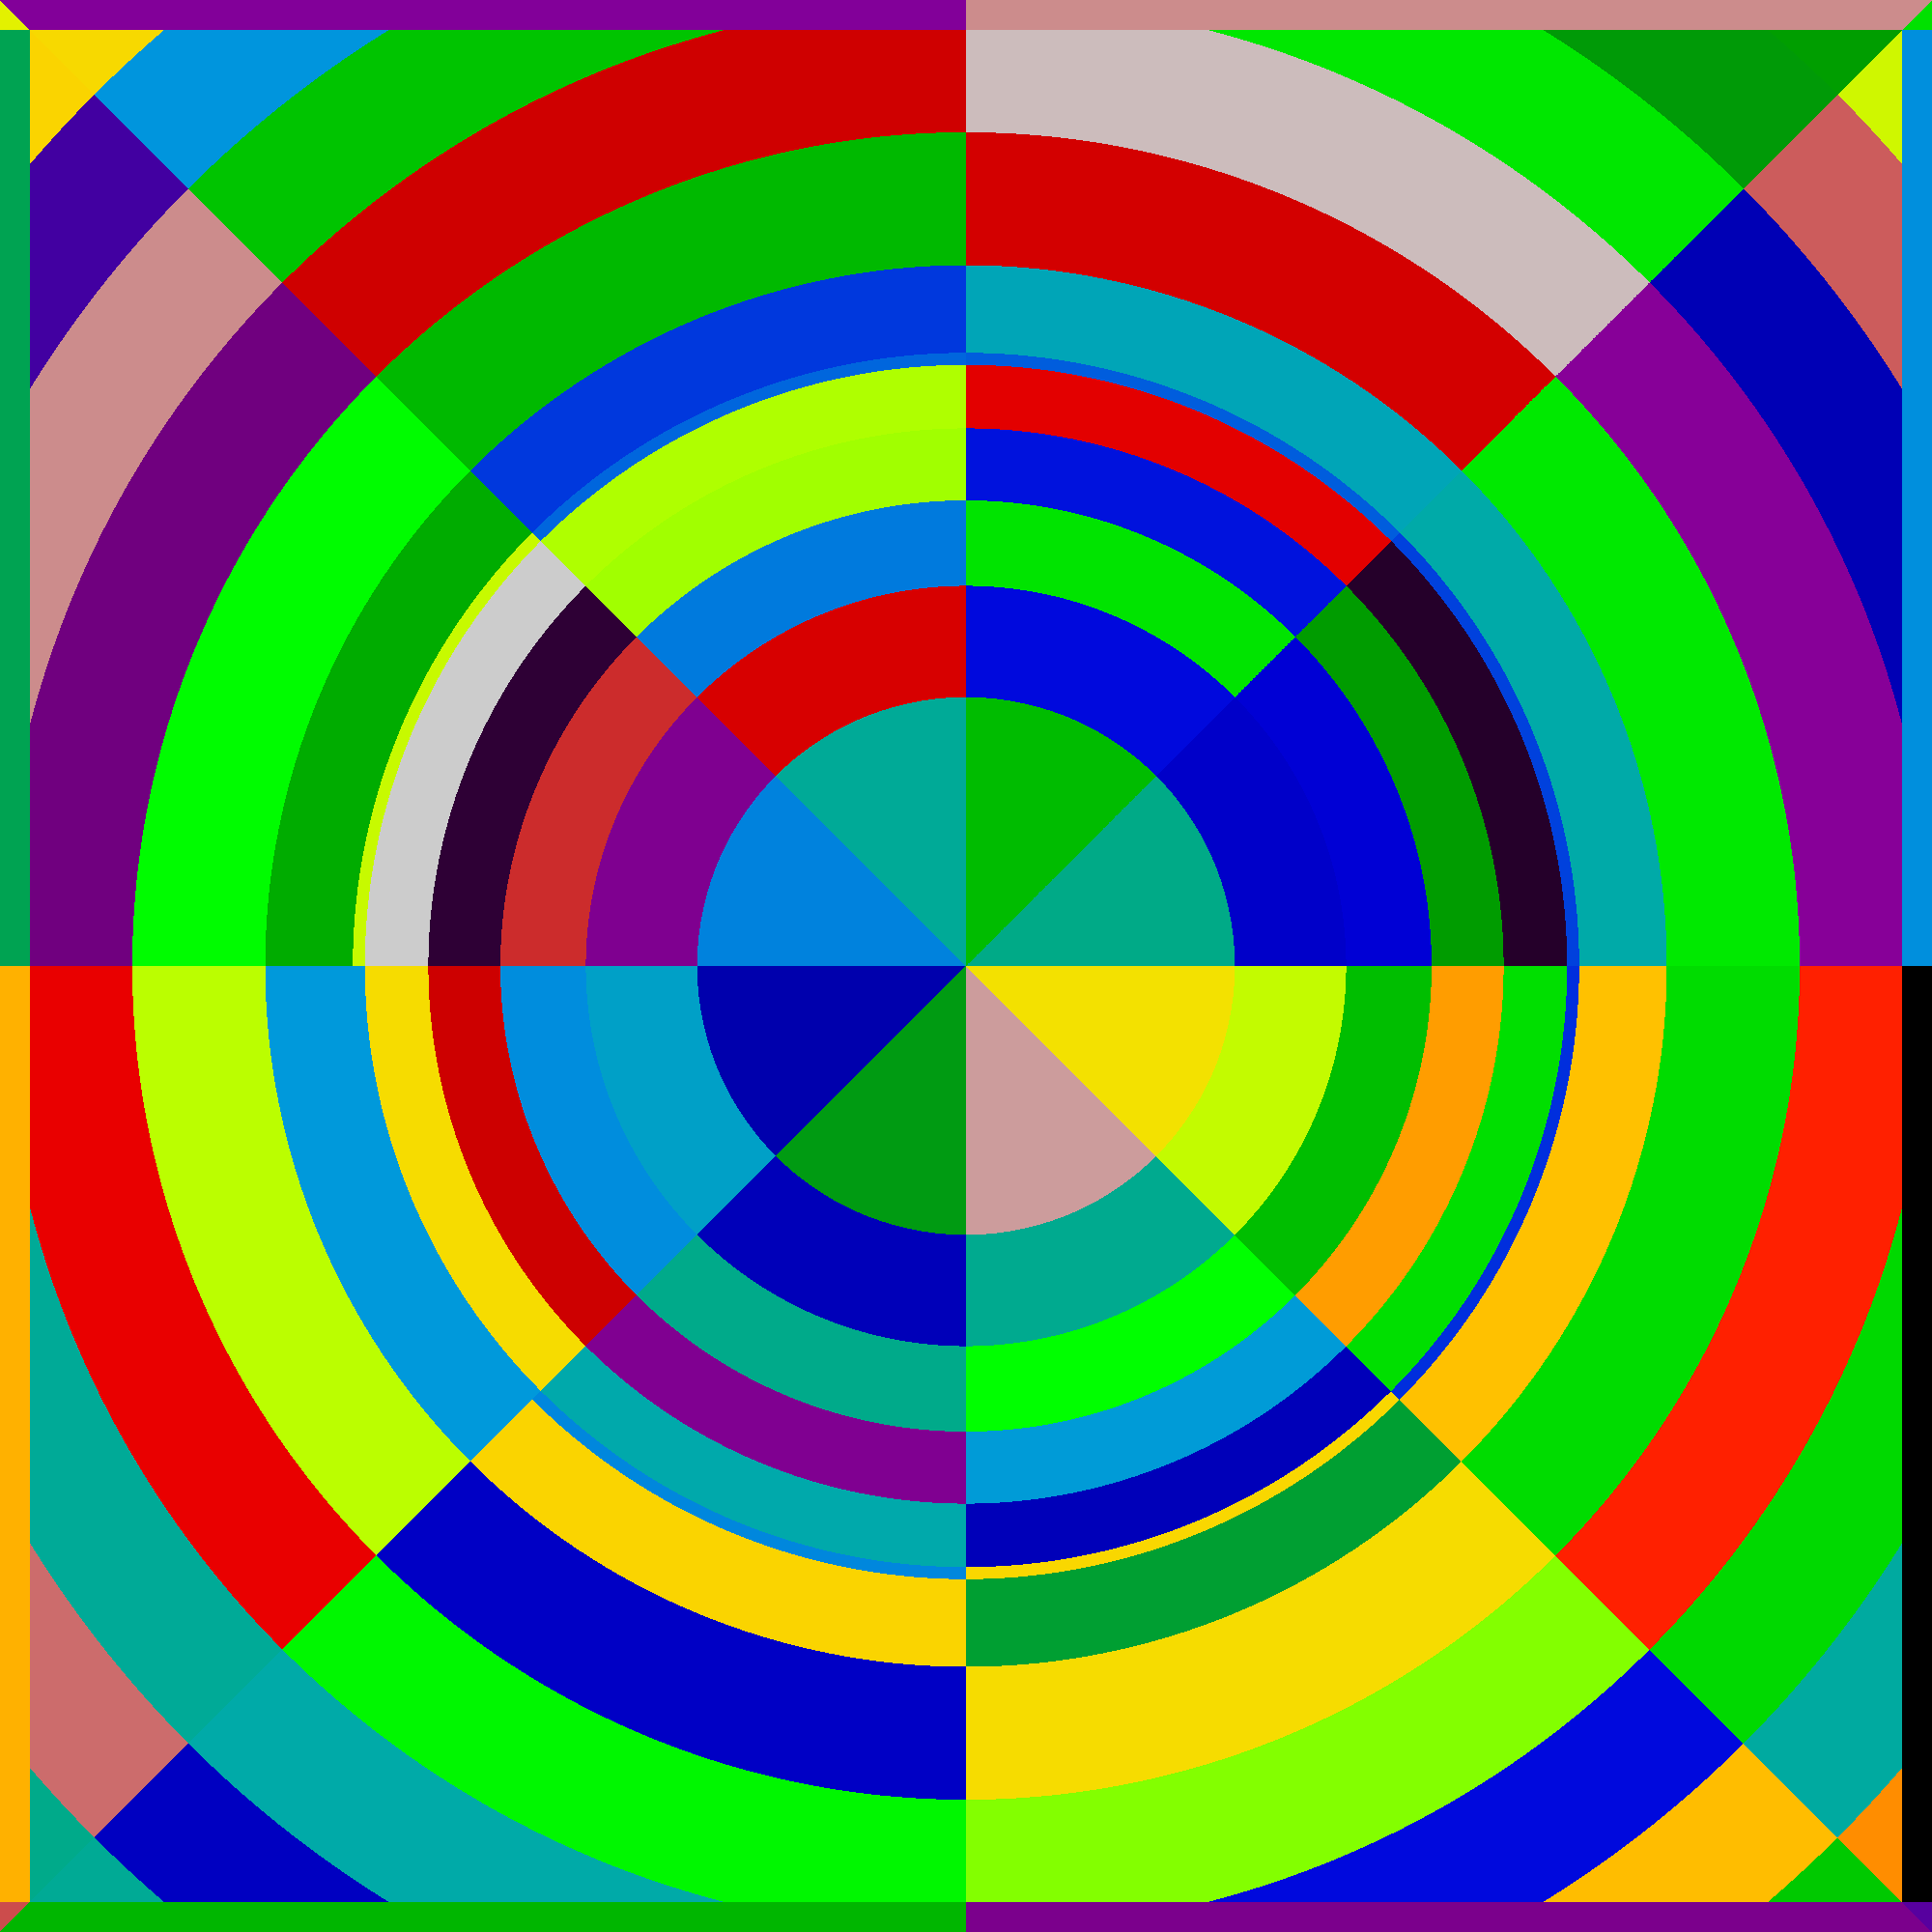
\includegraphics[width=0.9\linewidth]{figures/quantification/fsrs/fsrs-fuel-pin}
  \caption{}
  \label{fig:chap8-pin-1.6}
\end{subfigure}%
\begin{subfigure}{.5\textwidth}
  \centering
  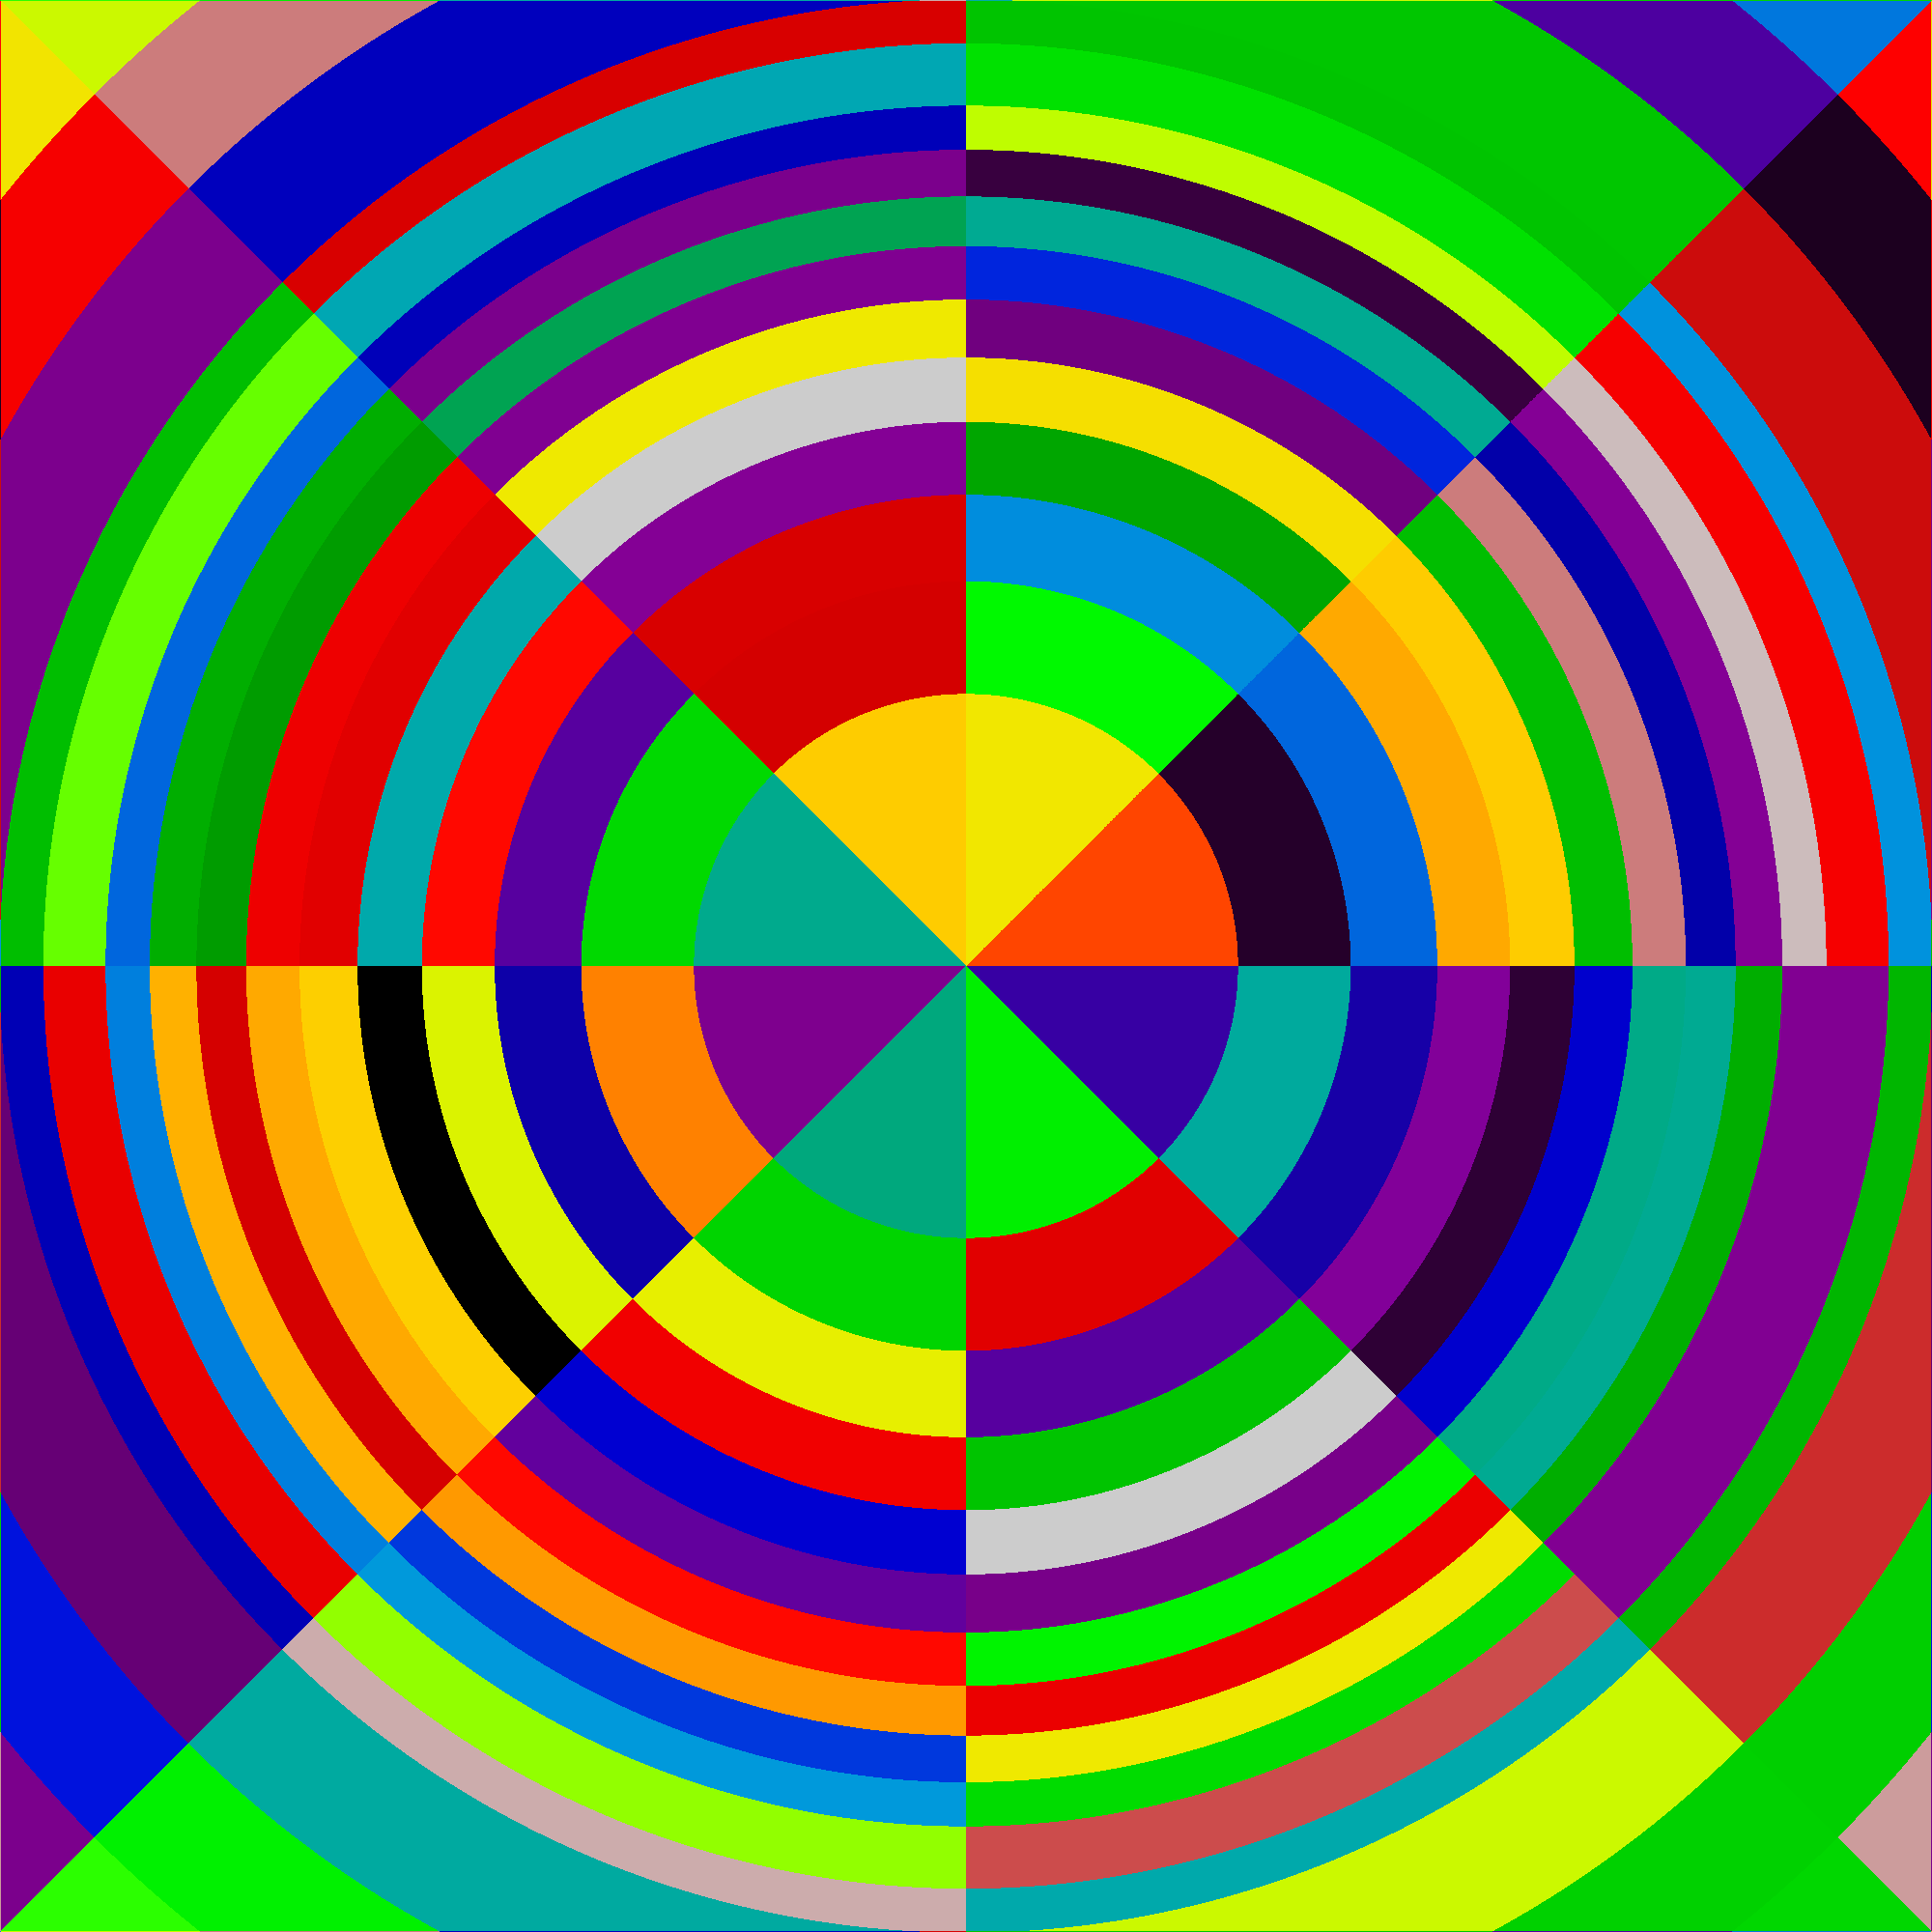
\includegraphics[width=0.9\linewidth]{figures/quantification/fsrs/fsrs-crgt}
  \caption{}
  \label{fig:chap8-pin-crgt}
\end{subfigure}
\begin{subfigure}{.5\textwidth}
  \centering
  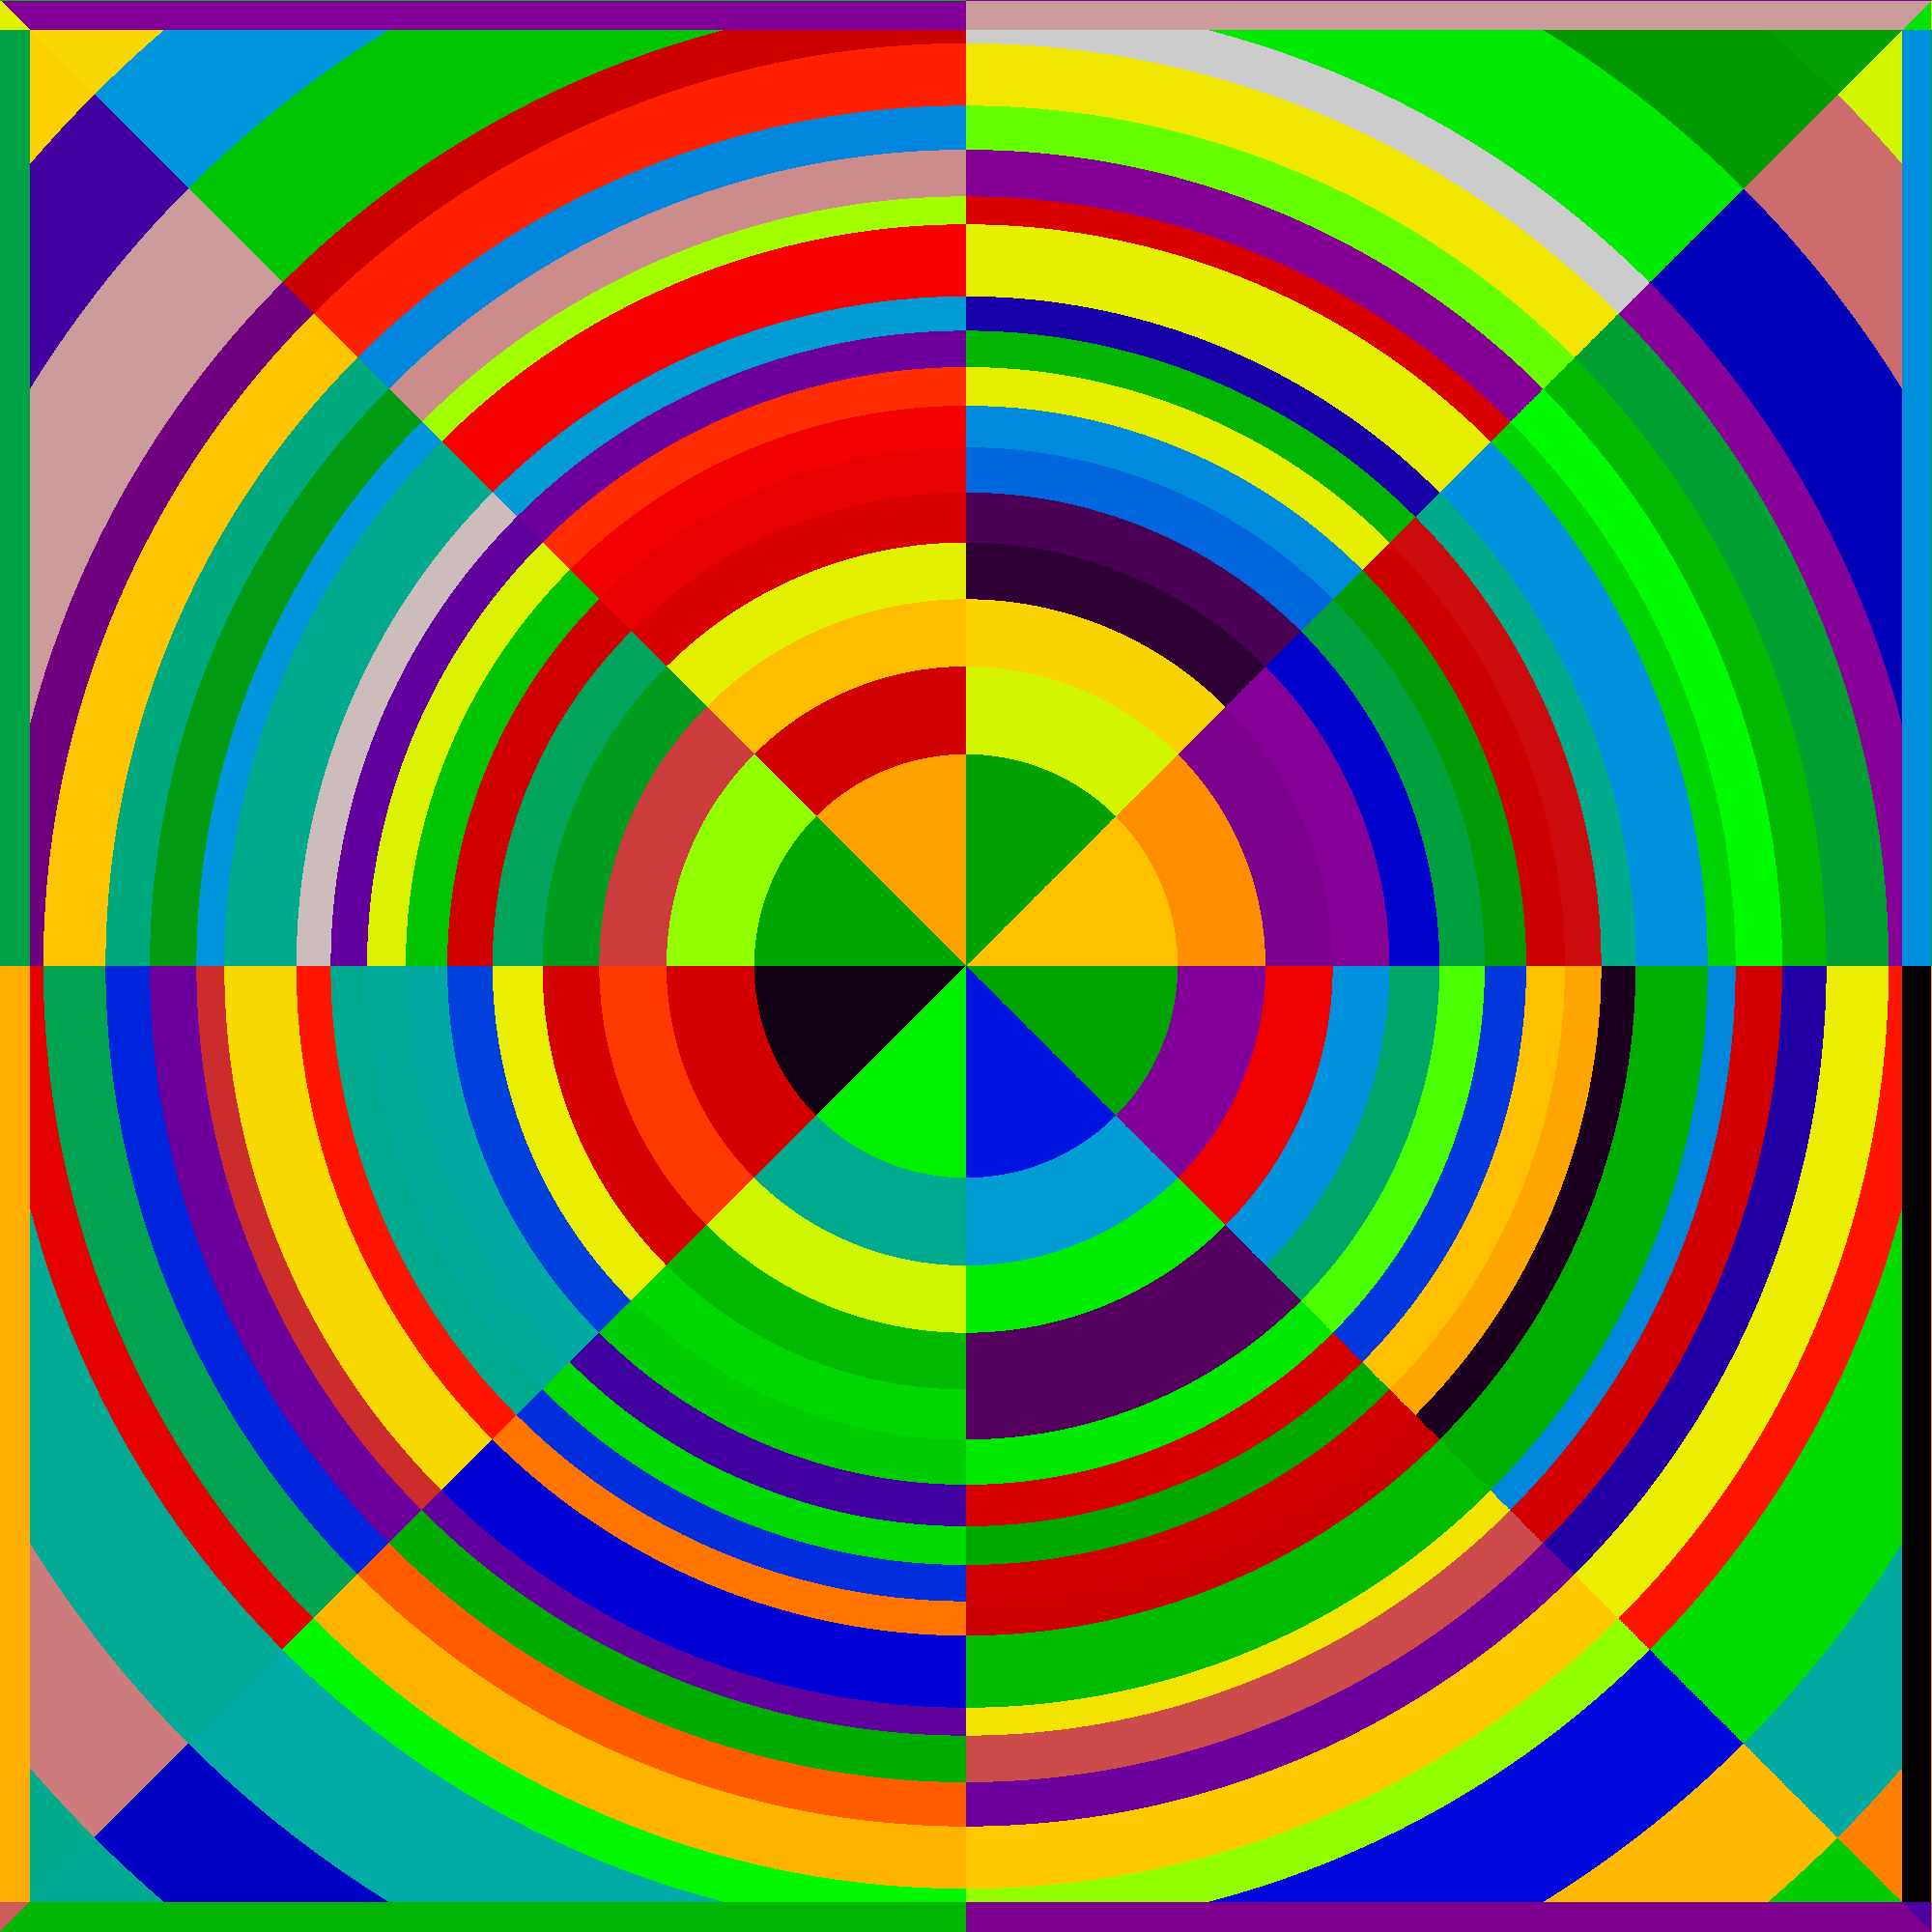
\includegraphics[width=0.9\linewidth]{figures/quantification/fsrs/fsrs-instr-tube}
  \caption{}
  \label{fig:chap8-instr-tube}
\end{subfigure}%
\begin{subfigure}{.5\textwidth}
  \centering
  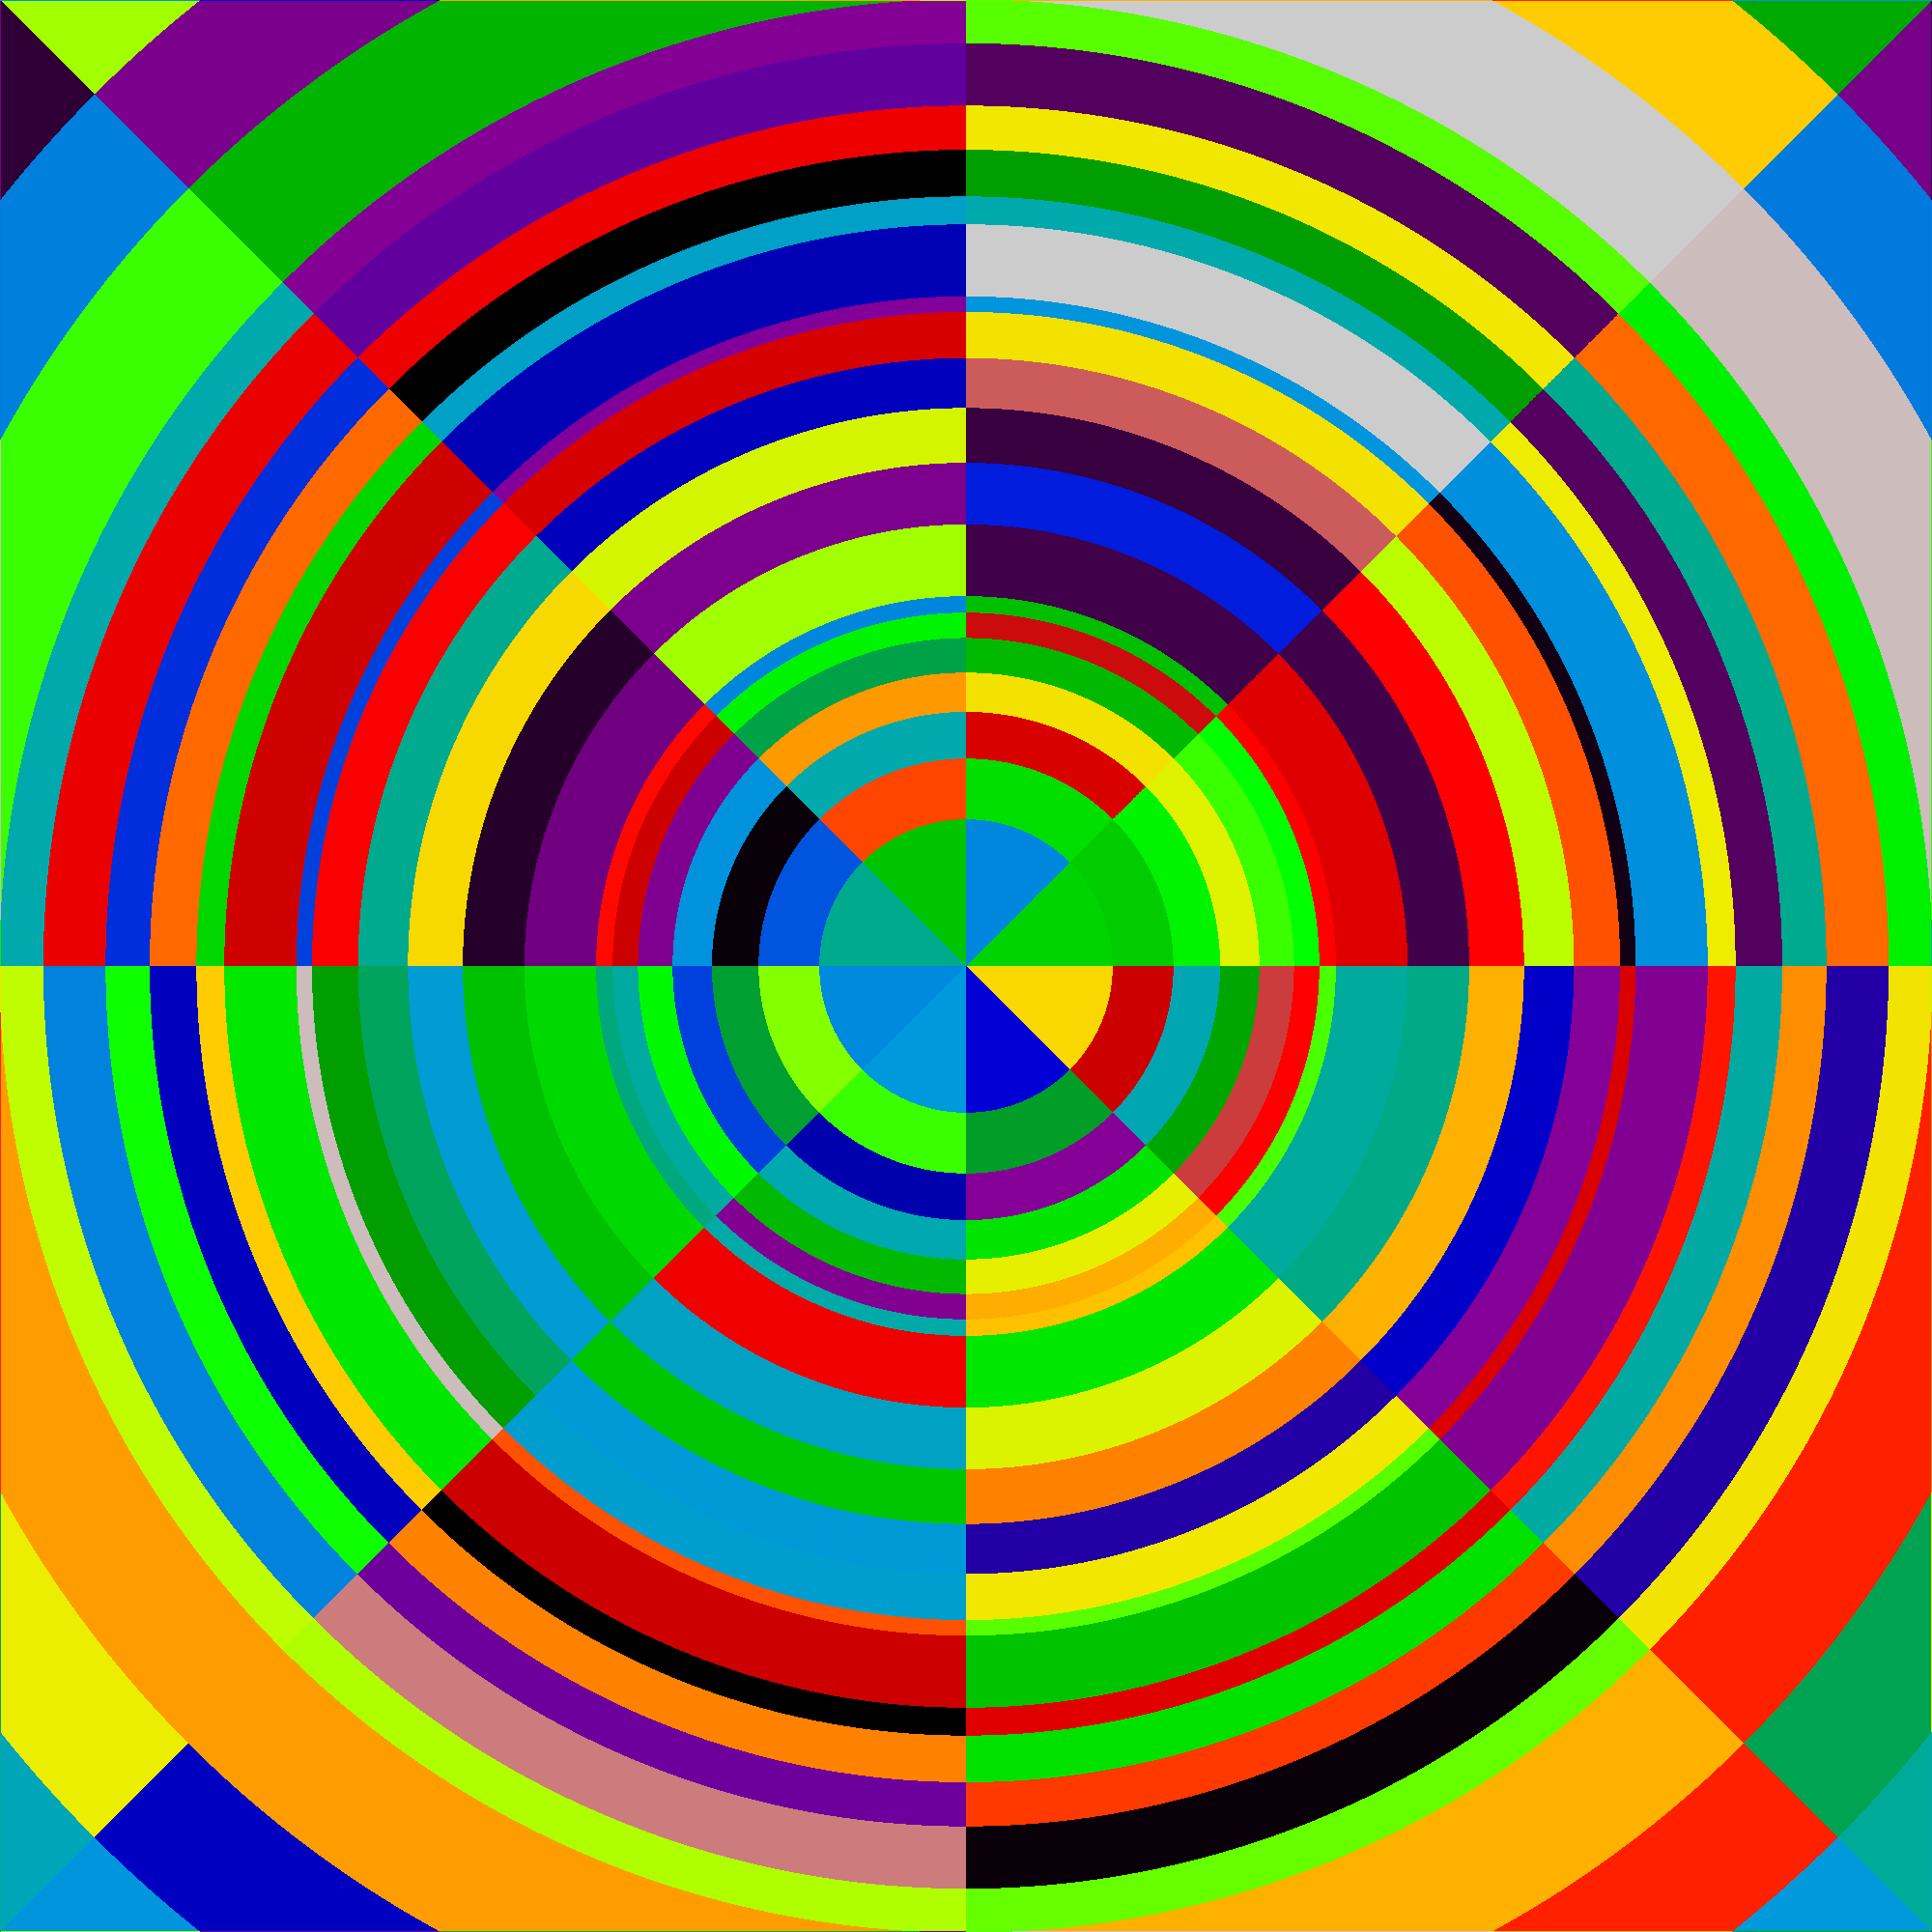
\includegraphics[width=0.9\linewidth]{figures/quantification/fsrs/fsrs-bp}
  \caption{}
  \label{fig:chap8-bp}
\end{subfigure}%
\caption[BEAVRS pin cell FSR discretization]{1.6\% enriched fuel pin (a), control rod guide tube (b), instrument tube (c) and burnable poison (d).}
\label{fig:chap8-pin-cell-fsrs}
\end{figure}

\begin{figure}[h!]
\centering
\begin{subfigure}{0.5\textwidth}
  \centering
  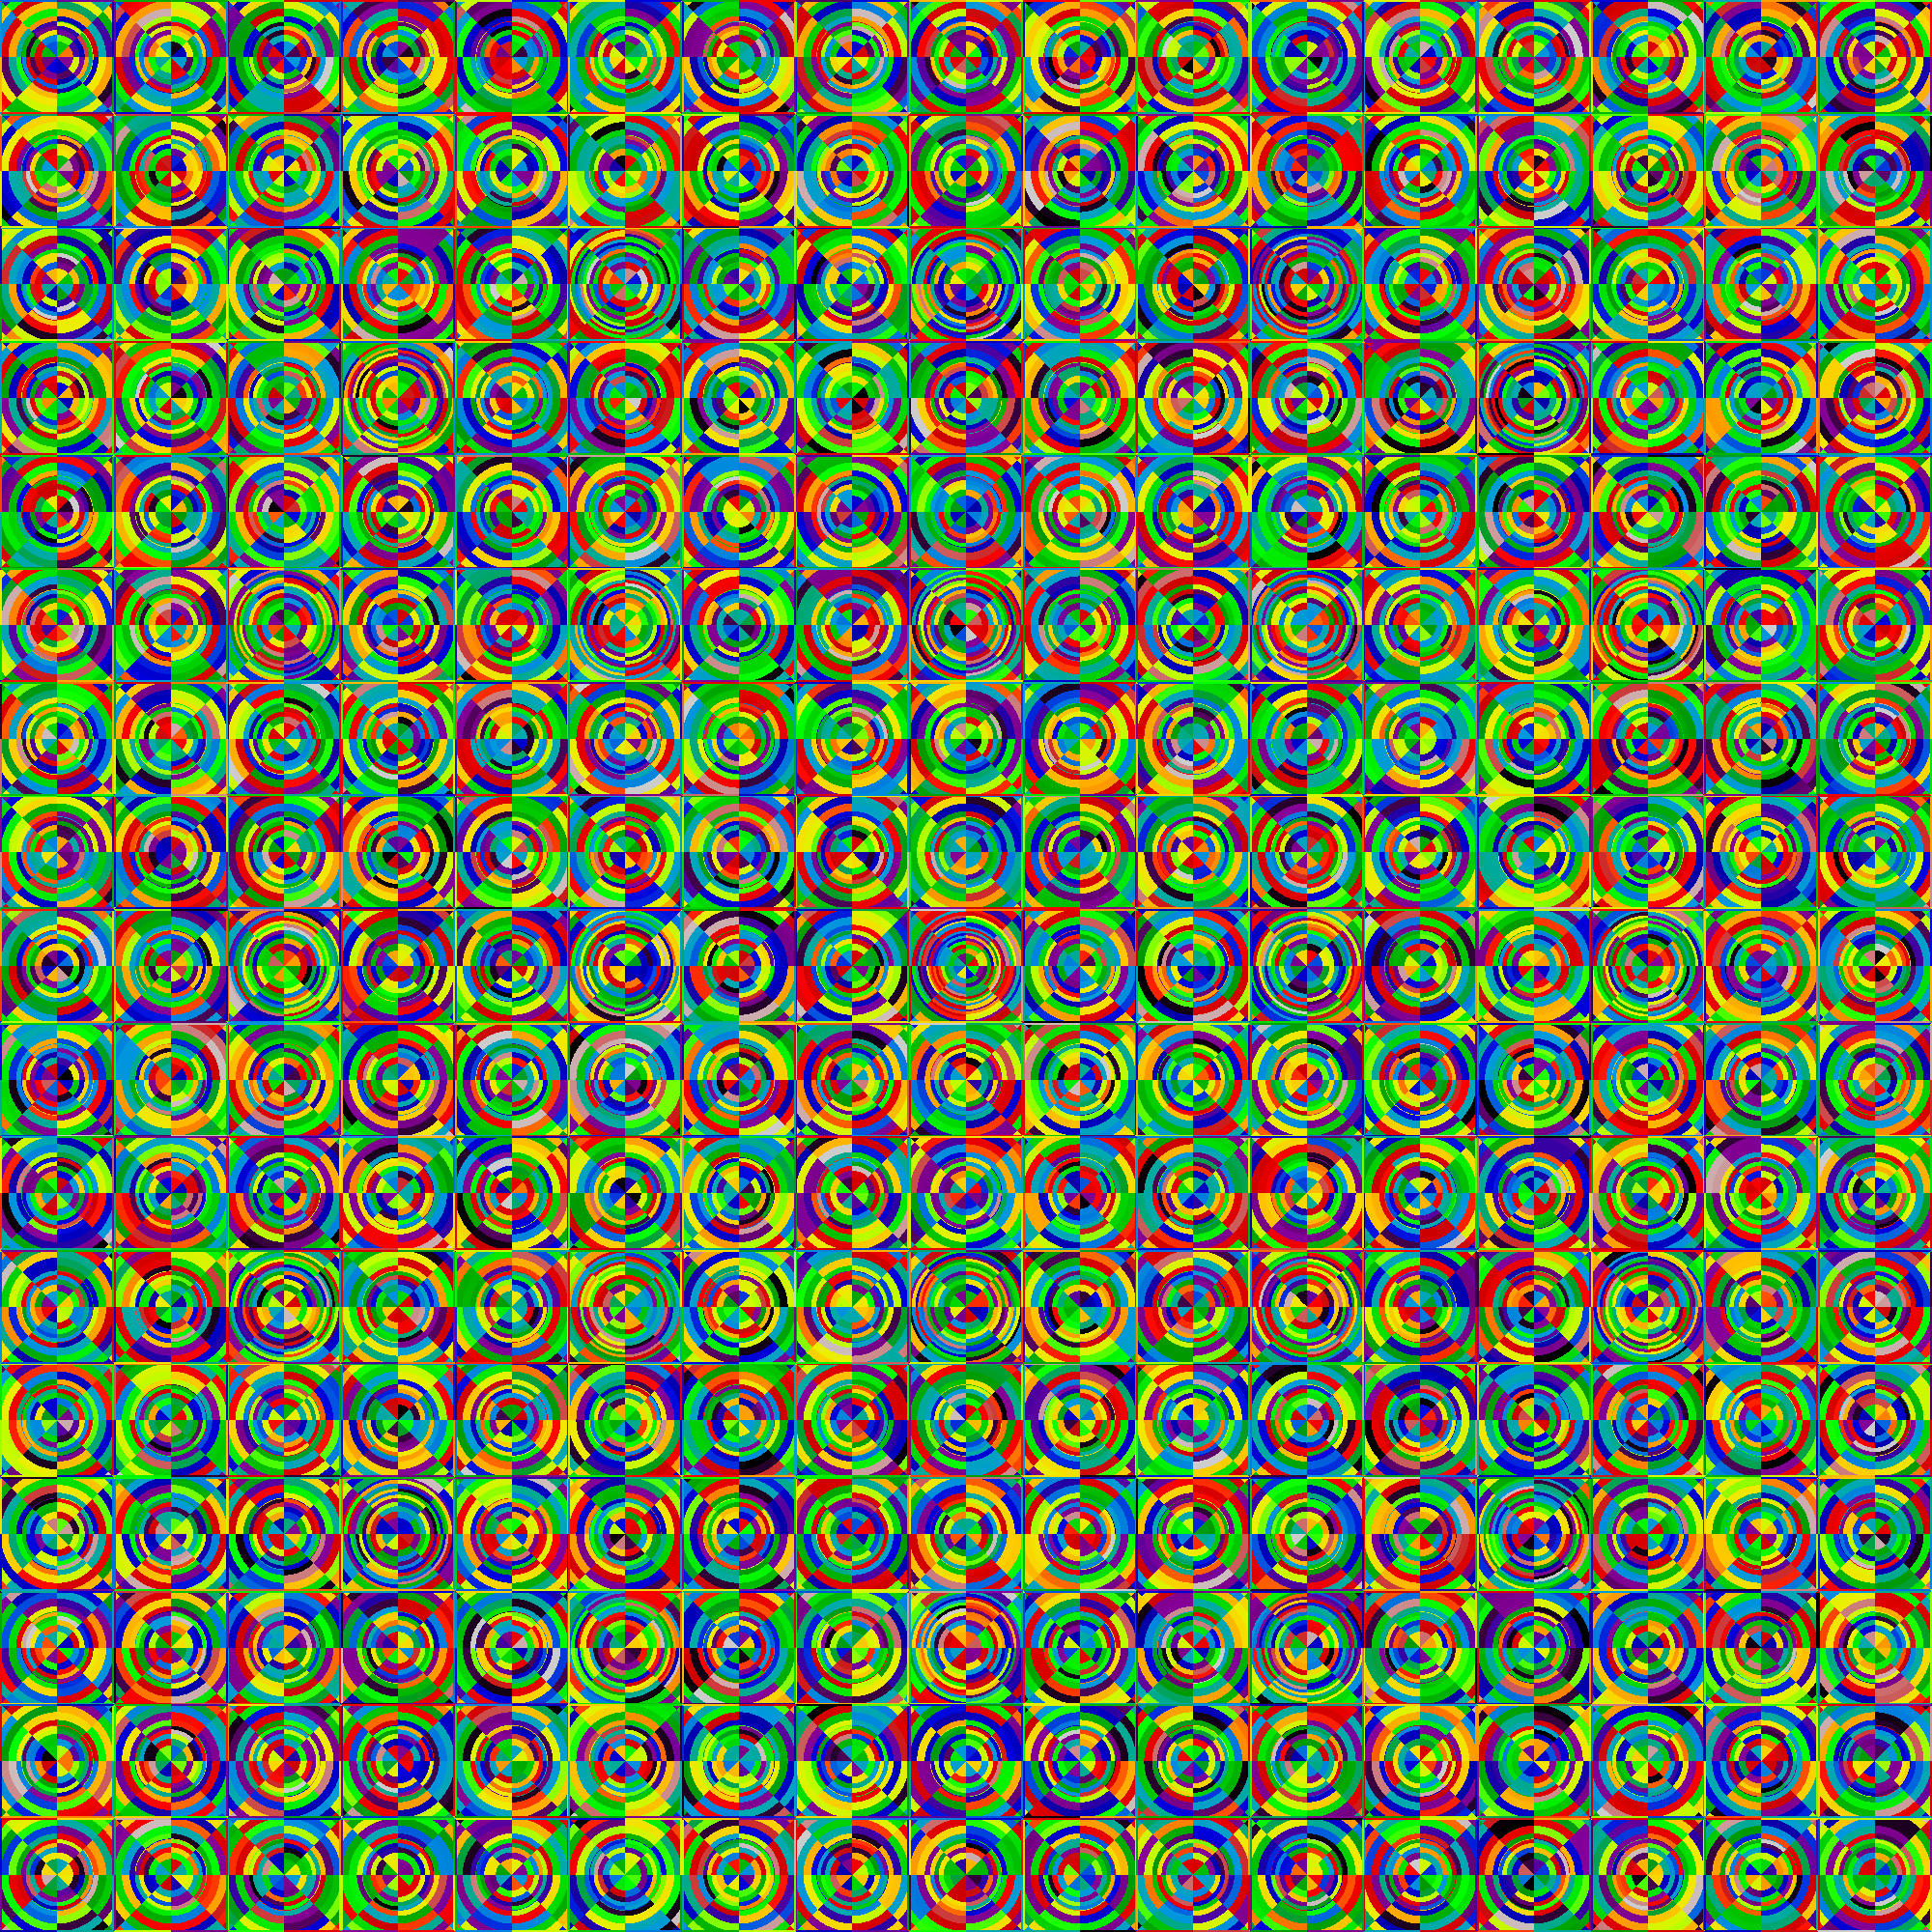
\includegraphics[width=0.9\linewidth]{figures/quantification/fsrs/fsrs-assm-16}
  \caption{}
  \label{fig:chap8-assm-1.6}
\end{subfigure}%
\begin{subfigure}{0.5\textwidth}
  \centering
  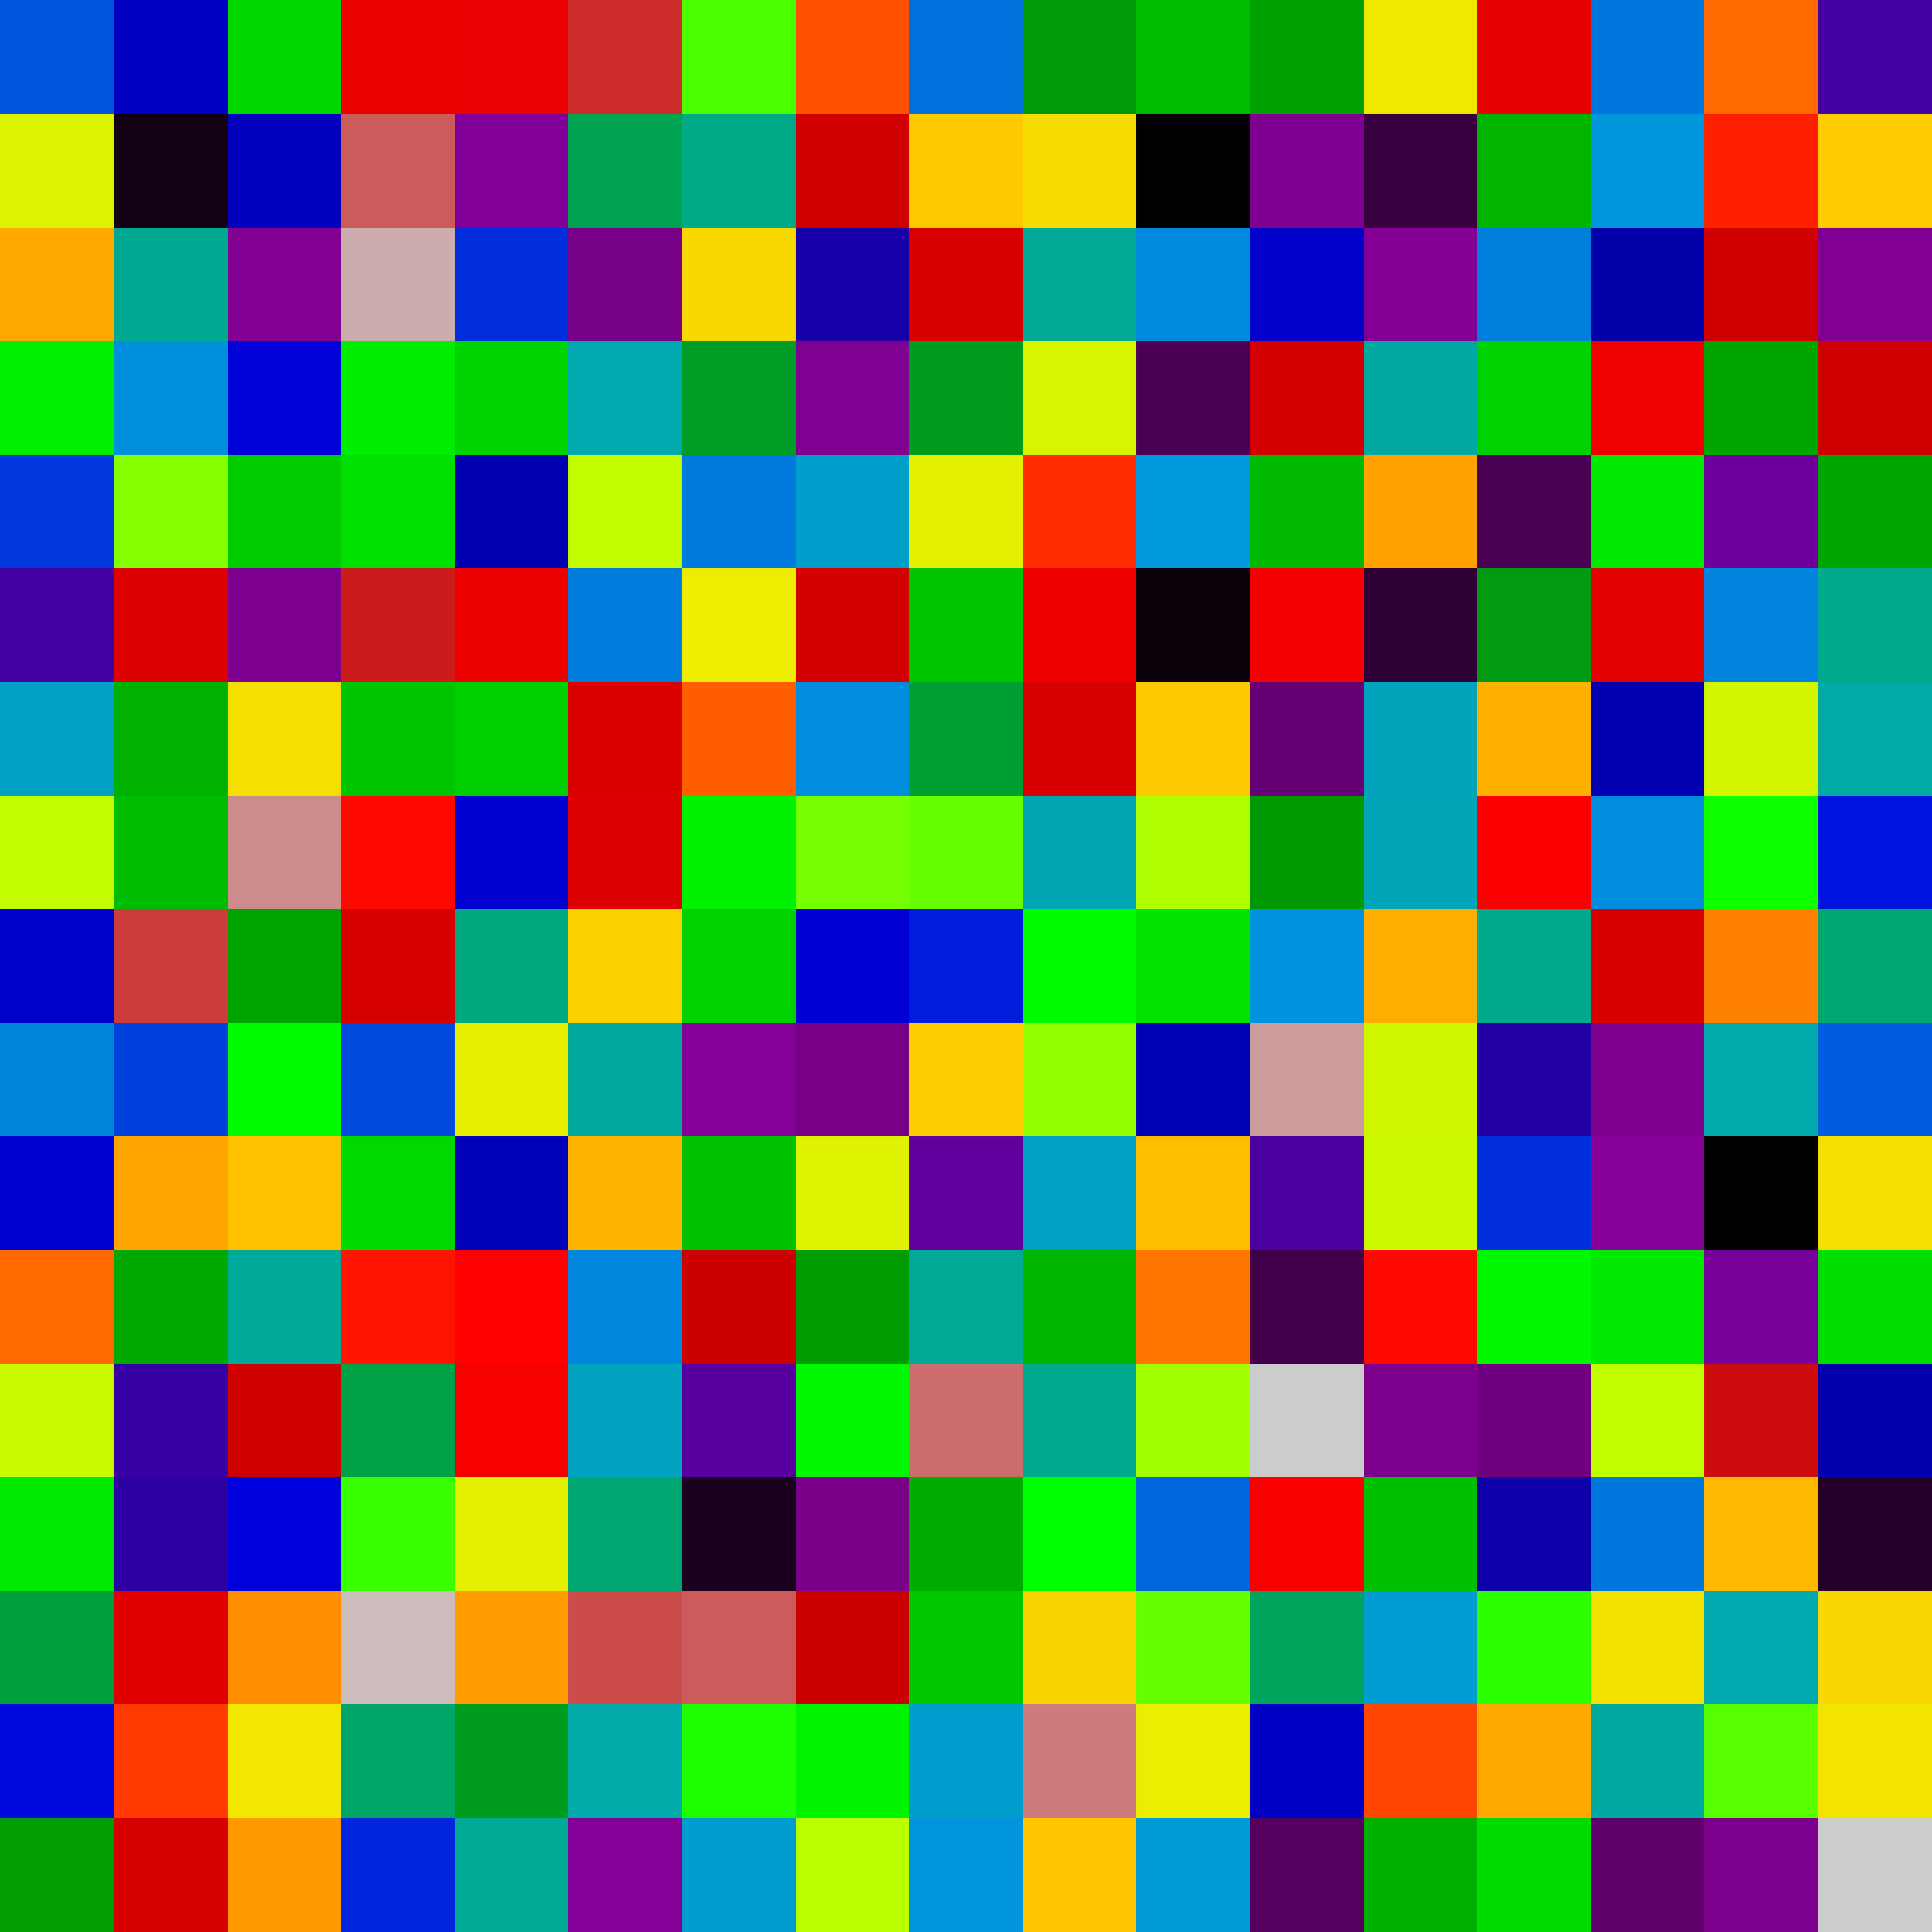
\includegraphics[width=0.9\linewidth]{figures/quantification/cmfd/cmfd-cells-assm}
  \caption{}
  \label{fig:chap8-cmfd-cells}
\end{subfigure}
\caption[FSR discretization and CMFD cells for a fuel assembly]{\ac{FSR} discretization and \ac{CMFD} cells for a fuel assembly}
\label{fig:chap8-assm-fsrs-cmfd-cells}
\end{figure}

\begin{figure}[h!]
\centering
\begin{subfigure}{0.5\textwidth}
  \centering
  
\includegraphics[width=0.9\linewidth]{figures/quantification/fsrs/fsrs-reflector}
  \caption{}
  \label{fig:chap8-assm-1.6}
\end{subfigure}%
\begin{subfigure}{0.5\textwidth}
  \centering
  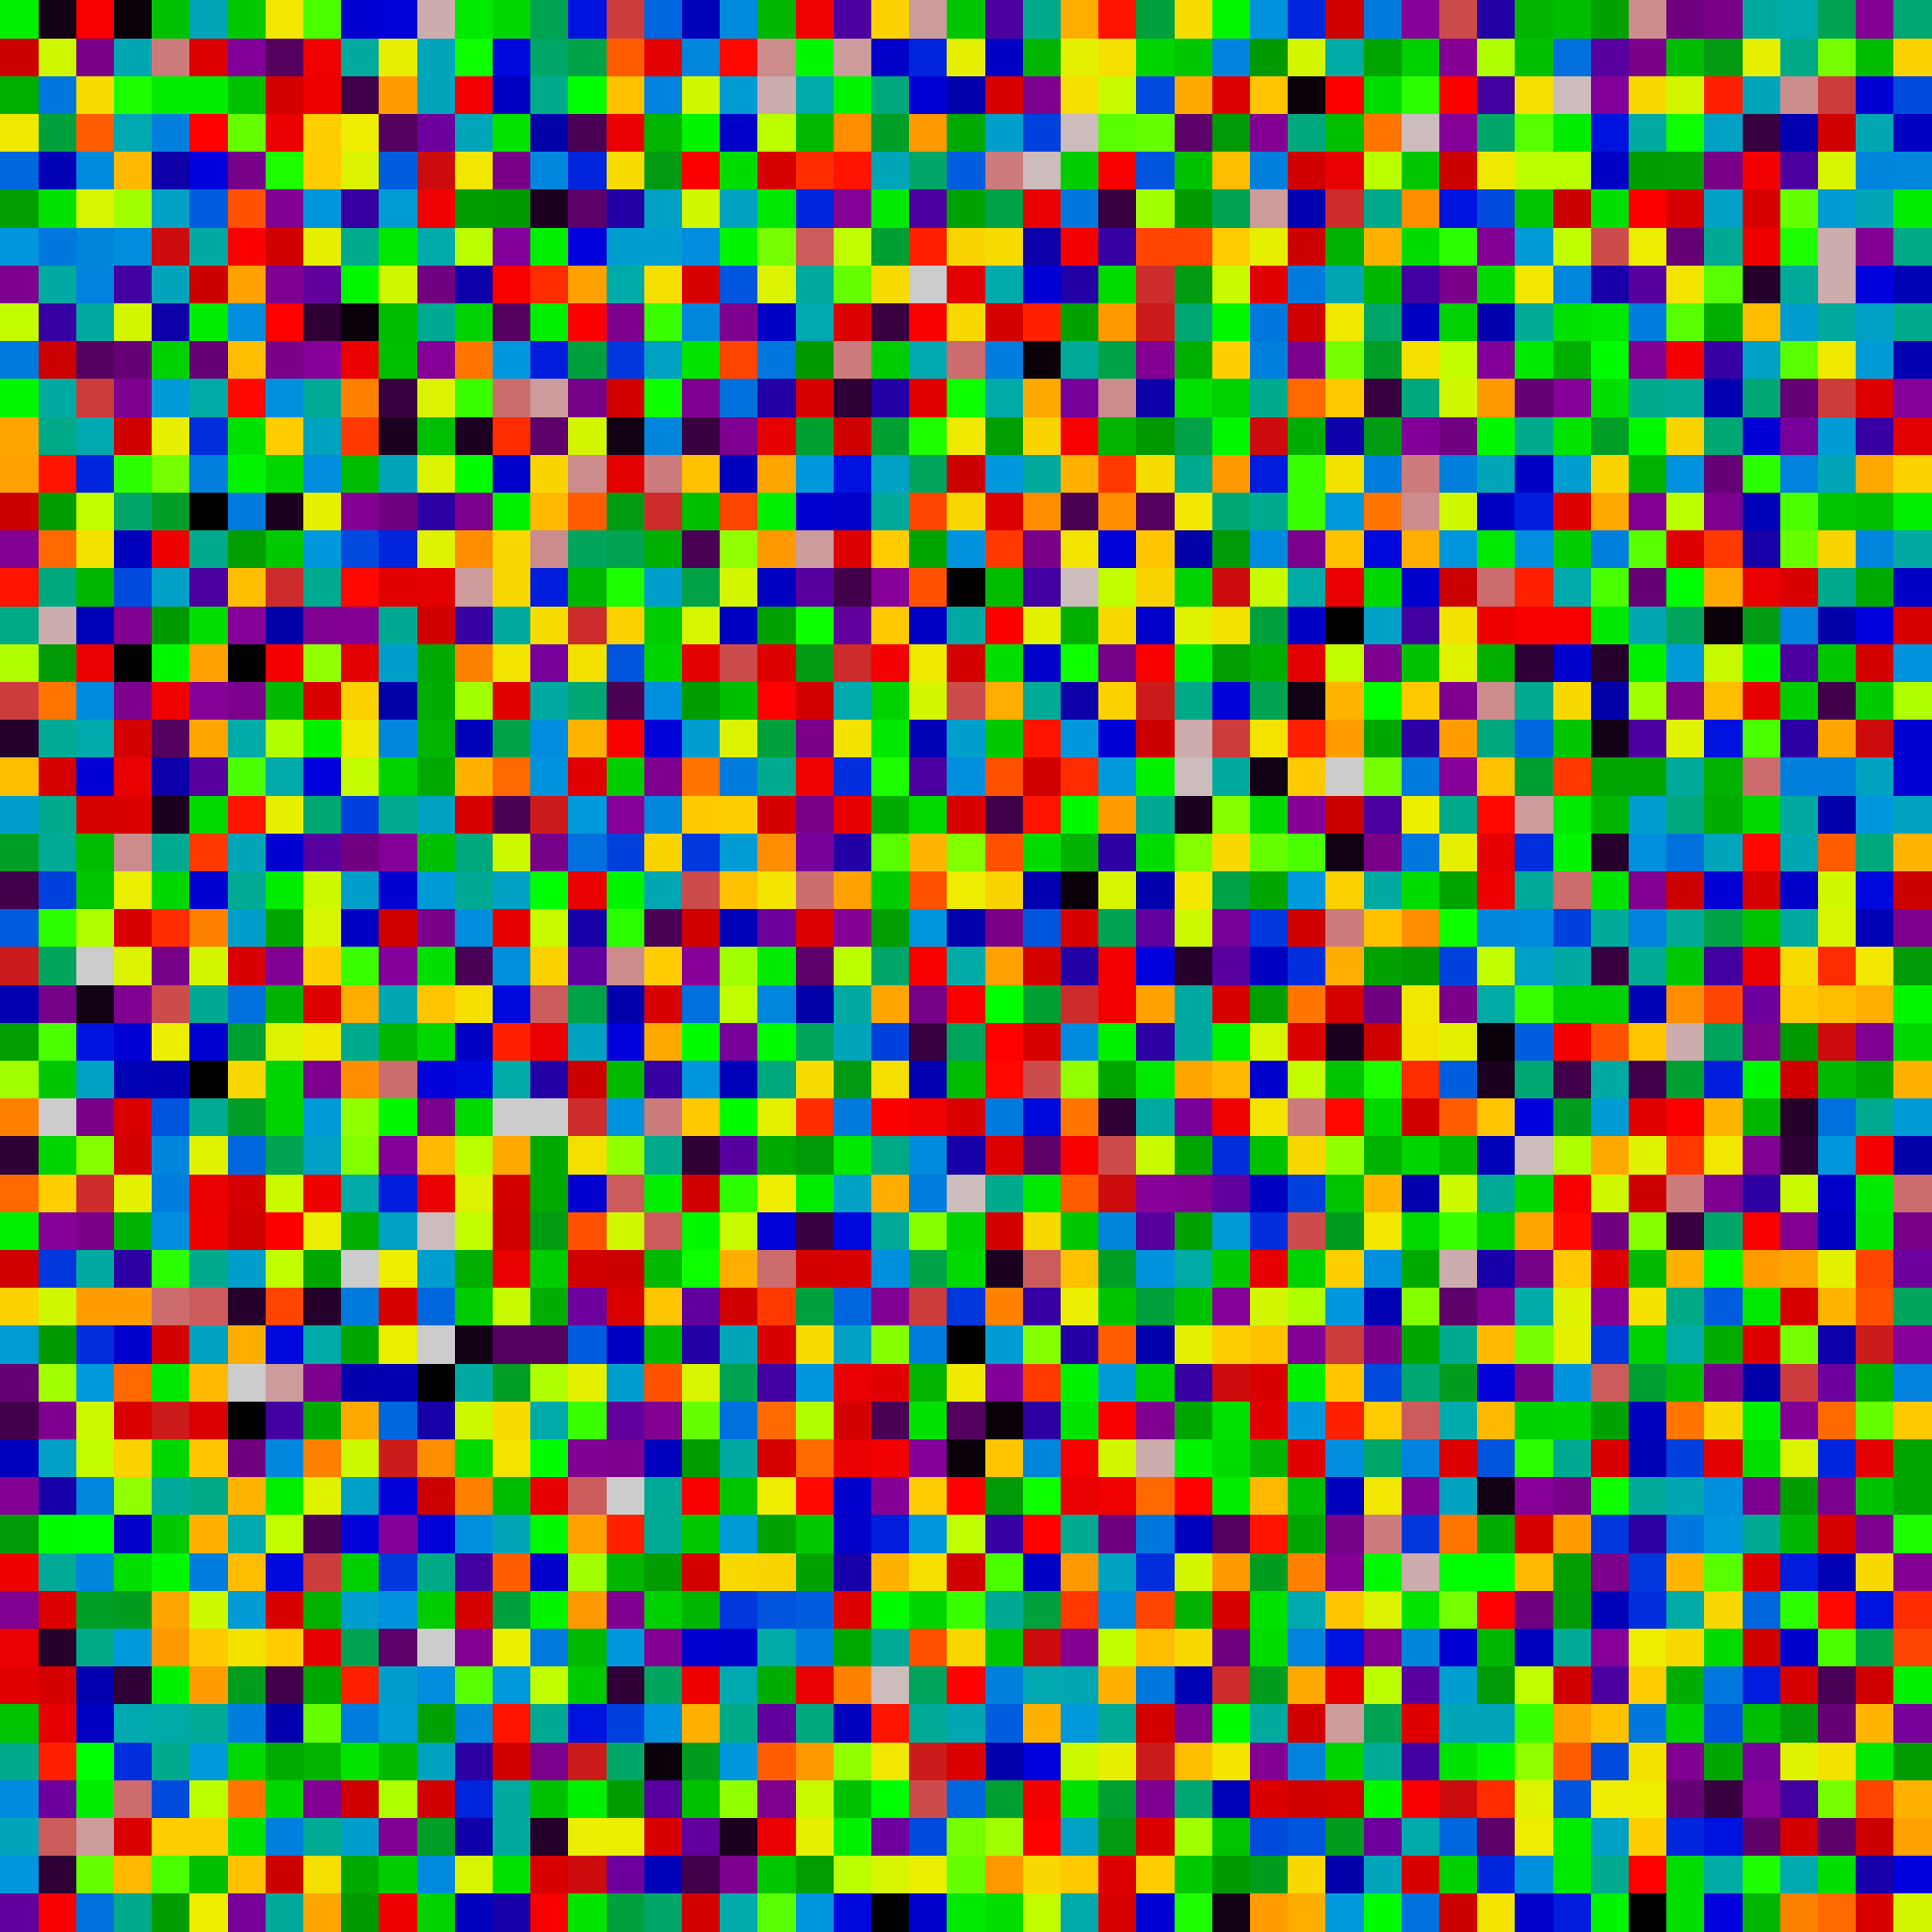
\includegraphics[width=0.9\linewidth]{figures/quantification/cmfd/cmfd-cells-reflector}
  \caption{}
  \label{fig:chap8-cmfd-cells}
\end{subfigure}
\caption[FSR discretization and CMFD cells for a 2$\times$2 colorset with a reflector]{\ac{FSR} discretization and \ac{CMFD} cells for a 2$\times$2 colorset with a water reflector.}
\label{fig:chap8-assm-fsrs-cmfd-cells}
\end{figure}

%%%%%%%%%%%%%%%%%%%%%%%%%%%%%%%%%%%%
\subsection{\ac{CMFD}}
\label{subsec:chap8-cmfd}

first paragraph:
-coarse pin-wise spatial mesh
-same energy group structure as in \ac{MOC}
-$k$-Nearest updated with 3 neighbors


%%%%%%%%%%%%%%%%%%%%%%%%%%%%%%%%%%%%%%%%%%%%%%%%%%%%%%%%%%%%%%%%%%%%%%%%%%%%%%%
\section{Analysis of Multi-Group Results}
\label{sec:chap8-mg-results}


%%%%%%%%%%%%%%%%%%%%%%%%
\subsection{Eigenvalues}
\label{subsec:chap8-eigenvalues}

\begin{table}[h!]
  \centering
  \caption[OpenMOC eigenvalue bias for heterogeneous benchmarks]{OpenMOC eigenvalue bias $\Delta\rho$ for heterogeneous benchmarks with varying spatial homogenization schemes and energy group structures.}
  \small
  \label{table:chap8-openmoc-eigenvalues}
  \vspace{6pt}
  \begin{tabular}{l l S[table-format=6.0] S[table-format=6.0] S[table-format=6.0]}
  \toprule
  \rowcolor{lightgray}
  & & \multicolumn{3}{S[table-format=6.1]}{\cellcolor{lightgray} {$\bm{\Delta\rho}$ \textbf{[pcm]}}} \\
  \multirow{-2}{*}{\cellcolor{lightgray} \bf Benchmark} &
  \multirow{-2}{*}{\cellcolor{lightgray} \bf \ac{MGXS} Scheme} &
  {\cellcolor{lightgray} \bf 2-Group} &
  {\cellcolor{lightgray} \bf 8-Group} &
  {\cellcolor{lightgray} \bf 70-Group} \\
  \midrule
\multirow{3}{*}{\parbox{2.5cm}{1.6\% Assm}} & Infinite & 217 & 3 & -163 \\
& Null & 83 & -50 & -136 \\
& Degenerate & 88 & -50 & -136 \\
  \midrule
\multirow{3}{*}{\parbox{2.5cm}{3.1\% Assm}} & Infinite & 180 & -34 & -195 \\
& Null & 93 & -54 & -159 \\
& Degenerate & 99 & -54 & -159 \\
  \midrule
\multirow{3}{*}{\parbox{2.5cm}{3.1\% Assm w/ 20 BPs}} & Infinite & 1056 & 151 & -270 \\
& Null & -143 & -157 & -227 \\
& Degenerate & -190 & -159 & -223 \\
  \midrule
\multirow{3}{*}{\parbox{2.5cm}{2$\times$2 Colorset}} & Infinite & 1022 & -22 & -229 \\
& Null & 16 & -79 & -183 \\
& Degenerate & -11 & -80 & -181 \\
  \midrule
\multirow{3}{*}{\parbox{2.5cm}{2$\times$2 Colorset w/ Reflector}} & Infinite & 2951 & 389 & -127 \\
& Null & 1477 & 474 & -109 \\
& Degenerate & 1394 & 482 & -98 \\
  \midrule
  \multirow{3}{*}{\parbox{2cm}{\ac{BEAVRS} Full Core}} & Infinite & 497 & 497 & \\
  & Null & & & \\
  & Degenerate & & & \\
  \bottomrule
\end{tabular}
\end{table}


%%%%%%%%%%%%%%%%%%%%%%%%%%
\subsection{Fission Rates}
\label{subsec:chap8-fiss-rates}

\begin{table}[h!]
  \centering
  \caption[Maximum OpenMOC fission rate errors]{Maximum OpenMOC fission rate errors for varying spatial homogenization schemes and energy groups structures.}
  \small
  \label{table:chap8-openmoc-max-fiss-rates}
  \vspace{6pt}
  \begin{tabular}{l l c c c}
  \toprule
  \rowcolor{lightgray}
  & & \multicolumn{3}{c}{\cellcolor{lightgray} \textbf{Max Error [\%]}} \\
  \multirow{-2}{*}{\cellcolor{lightgray} \bf Benchmark} &
  \multirow{-2}{*}{\cellcolor{lightgray} \bf \ac{MGXS} Scheme} &
  {\cellcolor{lightgray} \bf 2-Group} &
  {\cellcolor{lightgray} \bf 8-Group} &
  {\cellcolor{lightgray} \bf 70-Group} \\
  \midrule
\multirow{3}{*}{\parbox{2.5cm}{1.6\% Assm}} & Infinite & 2.76E+00 & 7.56E--01 & 4.71E--01 \\
& Null & 2.76E+00 & 7.46E--01 & 4.71E--01 \\
& Degenerate & 1.87E+00 & 7.83E--01 & 3.90E--01 \\
  \midrule
\multirow{3}{*}{\parbox{2.5cm}{3.1\% Assm}} & Infinite & 3.10E+00 & 8.29E--01 & 5.41E--01 \\
& Null & 3.09E+00 & 8.17E--01 & 5.42E--01 \\
& Degenerate & 2.09E+00 & 8.68E--01 & 4.72E--01 \\
  \midrule
\multirow{3}{*}{\parbox{2.5cm}{3.1\% Assm w/ 20 BPs}} & Infinite & -3.96E+00 & -9.41E--01 & 4.42E--01 \\
& Null & -4.02E+00 & -9.31E--01 & 4.44E--01 \\
& Degenerate & -1.88E+00 & -7.57E--01 & 3.70E--01 \\
  \midrule
\multirow{3}{*}{\parbox{2.5cm}{2$\times$2 Colorset}} & Infinite & 6.45E+00 & -1.52E+00 & 4.99E--01 \\
& Null & 6.17E+00 & -1.54E+00 & 5.34E--01 \\
& Degenerate & -4.62E+00 & -1.44E+00 & 5.00E--01 \\
  \midrule
\multirow{3}{*}{\parbox{2.5cm}{2$\times$2 Colorset w/ Reflector}} & Infinite & 1.24E+01 & 3.18E+00 & 8.37E--01 \\
& Null & -1.33E+01 & 2.96E+00 & 8.66E--01 \\
& Degenerate & 1.01E+01 & 2.59E+00 & 7.97E--01 \\
  \midrule
  \multirow{3}{*}{\parbox{2cm}{\ac{BEAVRS} Full Core}} & Infinite & 497 & 497 & \\
  & Null & & & \\
  & Degenerate & & & \\
  \bottomrule
\end{tabular}
\end{table}

\begin{table}[h!]
  \centering
  \caption[Mean OpenMOC fission rate errors]{Mean OpenMOC fission rate errors for varying spatial homogenization schemes and energy groups structures.}
  \small
  \label{table:chap8-openmoc-mean-fiss-rates}
  \vspace{6pt}
  \begin{tabular}{l l c c c}
  \toprule
  \rowcolor{lightgray}
  & & \multicolumn{3}{c}{\cellcolor{lightgray} \textbf{Mean Error [\%]}} \\
  \multirow{-2}{*}{\cellcolor{lightgray} \bf Benchmark} &
  \multirow{-2}{*}{\cellcolor{lightgray} \bf \ac{MGXS} Scheme} &
  {\cellcolor{lightgray} \bf 2-Group} &
  {\cellcolor{lightgray} \bf 8-Group} &
  {\cellcolor{lightgray} \bf 70-Group} \\
  \midrule
\multirow{3}{*}{\parbox{2.5cm}{1.6\% Assm}} & Infinite & 5.09E--02 & 1.22E--02 & 7.47E--05 \\
& Null & 5.07E--02 & 1.20E--02 & 5.91E--05 \\
& Degenerate & 3.02E--02 & 1.09E--02 & 2.02E--03 \\
  \midrule
\multirow{3}{*}{\parbox{2.5cm}{3.1\% Assm}} & Infinite & 7.88E--02 & 1.89E--02 & 9.45E--04 \\
& Null & 7.81E--02 & 1.85E--02 & 8.94E--04 \\
& Degenerate & 4.50E--02 & 1.69E--02 & 3.36E--03 \\
  \midrule
\multirow{3}{*}{\parbox{2.5cm}{3.1\% Assm w/ 20 BPs}} & Infinite & 9.02E--02 & 1.55E--02 & 4.54E--03 \\
& Null & 8.83E--02 & 1.47E--02 & 4.45E--03 \\
& Degenerate & 1.71E--02 & 8.44E--03 & 4.15E--03 \\
  \midrule
\multirow{3}{*}{\parbox{2.5cm}{2$\times$2 Colorset}} & Infinite & 1.13E--02 & -1.11E--02 & -1.73E--03 \\
& Null & 3.55E--02 & -1.11E--02 & -2.88E--03 \\
& Degenerate & -1.03E--01 & -2.59E--02 & -3.73E--03 \\
  \midrule
\multirow{3}{*}{\parbox{2.5cm}{2$\times$2 Colorset w/ Reflector}} & Infinite & 1.22E+00 & 3.19E--01 & 3.66E--02 \\
& Null & 8.54E--01 & 2.42E--01 & 4.28E--02 \\
& Degenerate & 1.08E+00 & 2.07E--01 & 1.16E--02 \\
  \midrule
  \multirow{3}{*}{\parbox{2cm}{\ac{BEAVRS} Full Core}} & Infinite & 497 & 497 & \\
  & Null & & & \\
  & Degenerate & & & \\
  \bottomrule
\end{tabular}
\end{table}

\begin{figure}[h!]
\centering
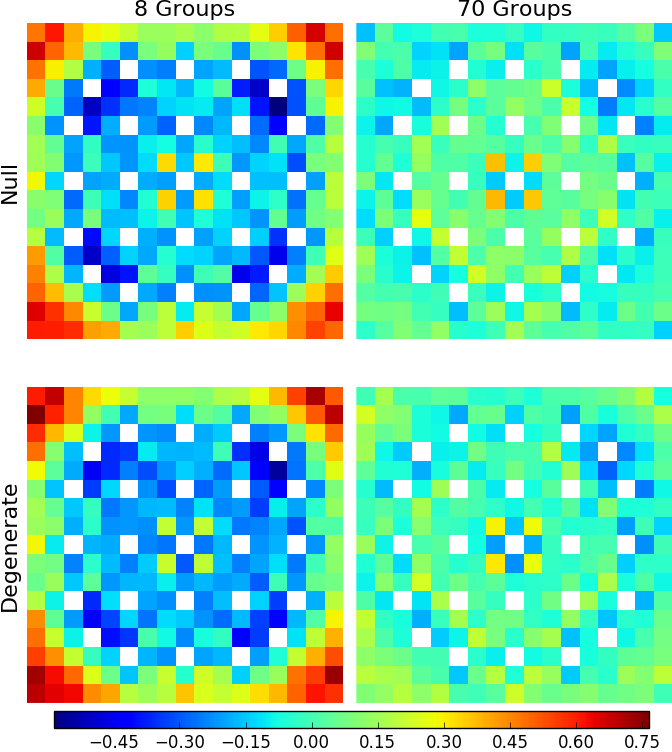
\includegraphics[width=\linewidth]{figures/quantification/assm-16/fiss-err}
\caption[Fission rate errors for a 1.6\% enriched assembly]{Fission rate errors for a 1.6\% enriched assembly.}
\label{fig:chap8-assm-1.6-fiss-err}
\end{figure}

\begin{figure}[h!]
\centering
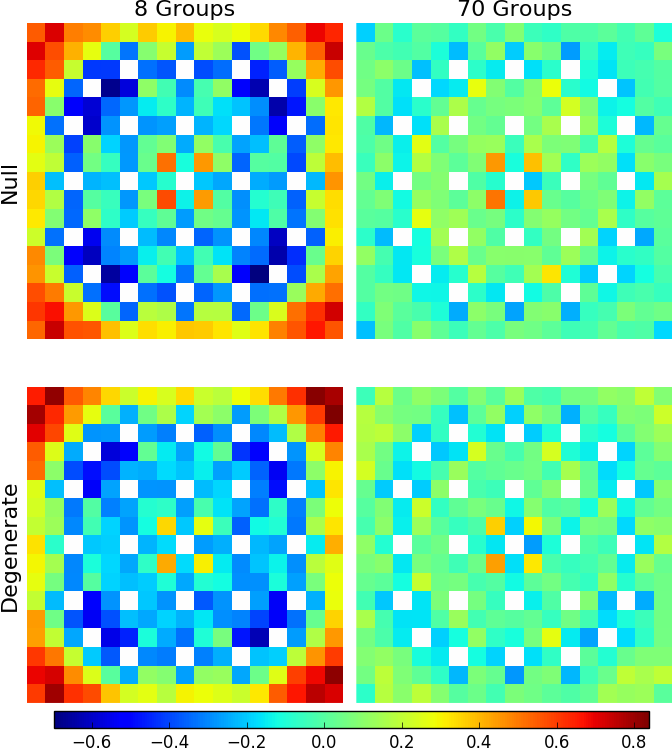
\includegraphics[width=\linewidth]{figures/quantification/assm-31/fiss-err}
\caption[Fission rate errors for a 3.1\% enriched assembly]{Fission rate errors for a 3.1\% enriched assembly.}
\label{fig:chap8-assm-3.1-fiss-err}
\end{figure}

\begin{figure}[h!]
\centering
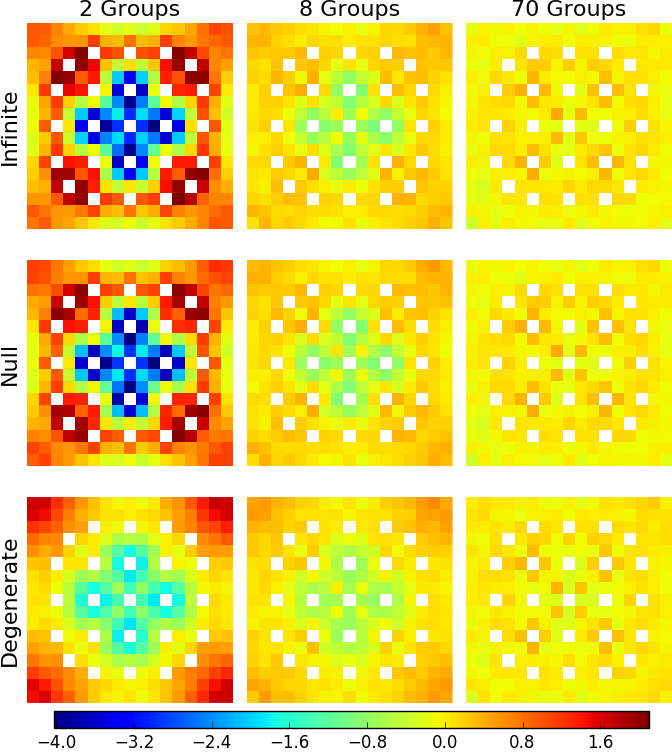
\includegraphics[width=\linewidth]{figures/quantification/assm-31-20BPs/fiss-err}
\caption[Fission rate errors for a 3.1\% enriched assembly with 20 BPs]{Fission rate errors for a 3.1\% enriched assembly with 20 BPs.}
\label{fig:chap8-assm-3.1-20BPs-fiss-err}
\end{figure}

\begin{figure}[h!]
\centering
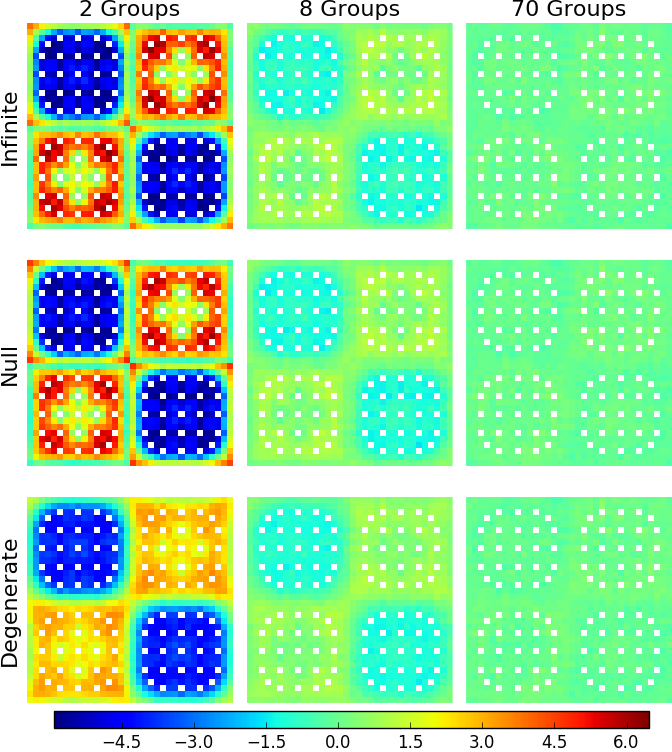
\includegraphics[width=\linewidth]{figures/quantification/2x2/fiss-err}
\caption[Fission rate errors for a 2$\times$2 colorset]{Fission rate errors for a 2$\times$2 colorset.}
\label{fig:chap8-2x2-fiss-err}
\end{figure}

\begin{figure}[h!]
\centering
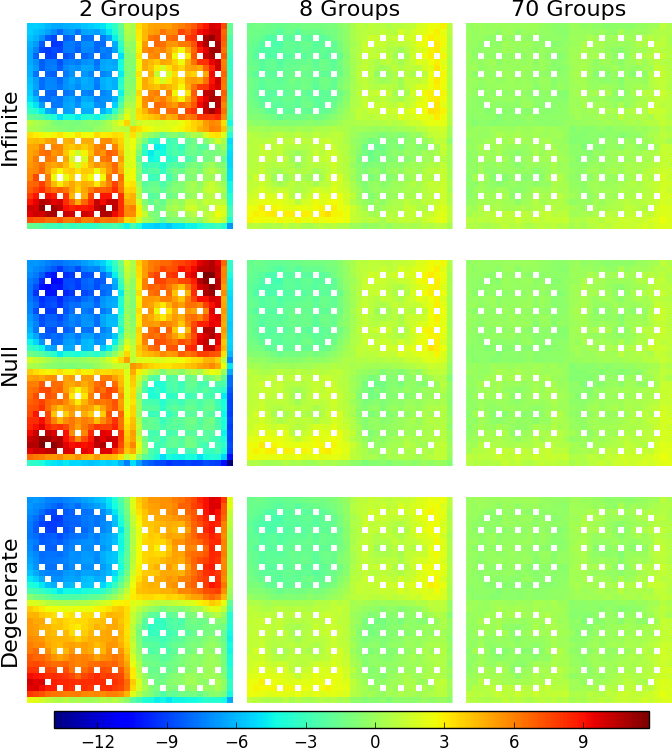
\includegraphics[width=\linewidth]{figures/quantification/reflector/fiss-err}
\caption[Fission rate errors for a 2$\times$2 colorset with a reflector]{Fission rate errors for a 2$\times$2 colorset with a reflector.}
\label{fig:chap8-reflector-fiss-err}
\end{figure}

\begin{figure}[h!]
\centering
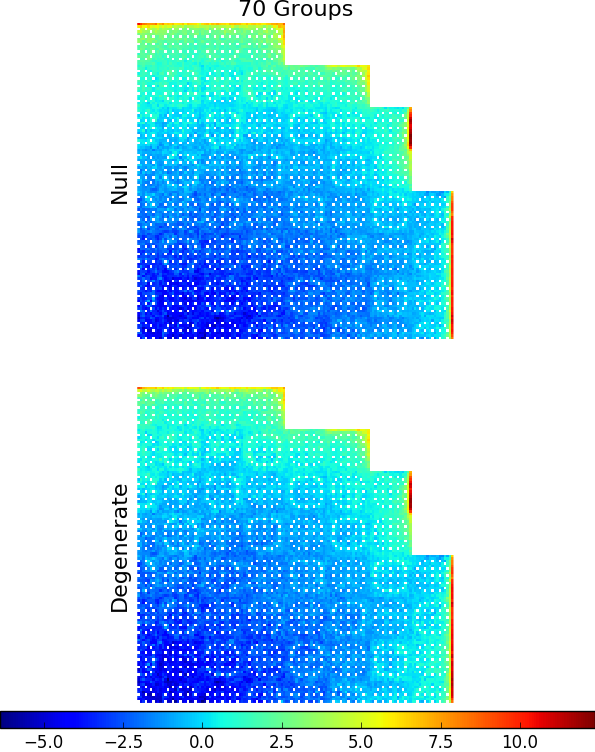
\includegraphics[width=\linewidth]{figures/quantification/full-core/fiss-err}
\caption[Fission rate errors for the 2D full core \ac{BEAVRS} model]{Fission rate errors for the 2D full core \ac{BEAVRS} model.}
\label{fig:chap8-full-core-fiss-err}
\end{figure}

\begin{itemize}[noitemsep]
  \item convergence rates for max/mean rel. err. for each benchmark
  \begin{itemize}[noitemsep]
    \item infinite vs. null vs. degenerate
    \item by energy group structure?
  \end{itemize}
  \item 2D heat maps of error distributions for each benchmark
  \begin{itemize}[noitemsep]
    \item infinite vs. null vs. degenerate
    \item by energy group structure?
  \end{itemize}
\end{itemize}

%%%%%%%%%%%%%%%%%%%%%%%%%%%%%%%%%%%%%%%%%%%%%
\subsection{U-238 Capture Rate Distributions}
\label{subsec:chap8-capt-rates}

\begin{table}[h!]
  \centering
  \caption[Maximum OpenMOC U-238 capture rate errors]{Maximum OpenMOC U-238 capture rate errors for varying spatial homogenization schemes and energy groups structures.}
  \small
  \label{table:chap8-openmoc-max-capt-rates}
  \vspace{6pt}
  \begin{tabular}{l l c c c}
  \toprule
  \rowcolor{lightgray}
  & & \multicolumn{3}{c}{\cellcolor{lightgray} \textbf{Max Error [\%]}} \\
  \multirow{-2}{*}{\cellcolor{lightgray} \bf Benchmark} &
  \multirow{-2}{*}{\cellcolor{lightgray} \bf \ac{MGXS} Scheme} &
  {\cellcolor{lightgray} \bf 2-Group} &
  {\cellcolor{lightgray} \bf 8-Group} &
  {\cellcolor{lightgray} \bf 70-Group} \\
  \midrule
\multirow{3}{*}{\parbox{2.5cm}{1.6\% Assm}} & Infinite & -2.86E+00 & -1.61E+00 & -1.17E+00 \\
& Null & -2.86E+00 & -1.60E+00 & -1.17E+00 \\
& Degenerate & 9.07E--01 & 3.88E--01 & 2.99E--01 \\
  \midrule
\multirow{3}{*}{\parbox{2.5cm}{3.1\% Assm}} & Infinite & -3.25E+00 & -1.91E+00 & -1.44E+00 \\
& Null & -3.24E+00 & -1.90E+00 & -1.44E+00 \\
& Degenerate & 8.14E--01 & 4.75E--01 & 3.39E--01 \\
  \midrule
\multirow{3}{*}{\parbox{2.5cm}{3.1\% Assm w/ 20 BPs}} & Infinite & 3.00E+00 & -1.30E+00 & -1.04E+00 \\
& Null & 3.02E+00 & -1.29E+00 & -1.04E+00 \\
& Degenerate & 1.36E+00 & 6.19E--01 & 2.96E--01 \\
  \midrule
\multirow{3}{*}{\parbox{2.5cm}{2$\times$2 Colorset}} & Infinite & -4.92E+00 & -2.09E+00 & -1.65E+00 \\
& Null & -4.52E+00 & -1.90E+00 & -1.59E+00 \\
& Degenerate & -2.12E+00 & -7.11E--01 & 4.75E--01 \\
  \midrule
\multirow{3}{*}{\parbox{2.5cm}{2$\times$2 Colorset w/ Reflector}} & Infinite & 1.27E+01 & 4.84E+00 & -2.42E+00 \\
& Null & 1.17E+01 & 3.74E+00 & -2.47E+00 \\
& Degenerate & 9.67E+00 & 3.28E+00 & -7.08E--01 \\
  \midrule
  \multirow{3}{*}{\parbox{2cm}{\ac{BEAVRS} Full Core}} & Infinite & 497 & 497 & \\
  & Null & & & \\
  & Degenerate & & & \\
  \bottomrule
\end{tabular}
\end{table}

\begin{table}[h!]
  \centering
  \caption[Mean OpenMOC U-238 capture rate errors]{Mean OpenMOC U-238 capture rate errors for varying spatial homogenization schemes and energy groups structures.}
  \small
  \label{table:chap8-openmoc-mean-capt-rates}
  \vspace{6pt}
  \begin{tabular}{l l c c c}
  \toprule
  \rowcolor{lightgray}
  & & \multicolumn{3}{c}{\cellcolor{lightgray} \textbf{Mean Error [\%]}} \\
  \multirow{-2}{*}{\cellcolor{lightgray} \bf Benchmark} &
  \multirow{-2}{*}{\cellcolor{lightgray} \bf \ac{MGXS} Scheme} &
  {\cellcolor{lightgray} \bf 2-Group} &
  {\cellcolor{lightgray} \bf 8-Group} &
  {\cellcolor{lightgray} \bf 70-Group} \\
  \midrule
\multirow{3}{*}{\parbox{2.5cm}{1.6\% Assm}} & Infinite & 3.41E--02 & 1.65E--02 & 1.17E--02 \\
& Null & 3.41E--02 & 1.65E--02 & 1.17E--02 \\
& Degenerate & 8.19E--03 & 5.01E--04 & 4.37E--04 \\
  \midrule
\multirow{3}{*}{\parbox{2.5cm}{3.1\% Assm}} & Infinite & 3.95E--02 & 1.98E--02 & 1.46E--02 \\
& Null & 3.94E--02 & 1.98E--02 & 1.46E--02 \\
& Degenerate & 8.15E--03 & -2.87E--04 & 4.77E--04 \\
  \midrule
\multirow{3}{*}{\parbox{2.5cm}{3.1\% Assm w/ 20 BPs}} & Infinite & -8.62E--03 & -3.80E--03 & -2.13E--03 \\
& Null & -7.91E--03 & -3.75E--03 & -2.17E--03 \\
& Degenerate & -3.50E--03 & -3.00E--03 & 2.29E--04 \\
  \midrule
\multirow{3}{*}{\parbox{2.5cm}{2$\times$2 Colorset}} & Infinite & 1.68E--01 & 1.71E--02 & 1.67E--02 \\
& Null & 1.28E--01 & 1.71E--03 & 1.13E--02 \\
& Degenerate & 9.91E--02 & -8.60E--03 & 6.92E--03 \\
  \midrule
\multirow{3}{*}{\parbox{2.5cm}{2$\times$2 Colorset w/ Reflector}} & Infinite & 1.90E+00 & 4.42E--01 & -2.59E--02 \\
& Null & 1.54E+00 & 3.60E--01 & -2.21E--02 \\
& Degenerate & 1.78E+00 & 4.42E--01 & 9.53E--03 \\
  \midrule
  \multirow{3}{*}{\parbox{2cm}{\ac{BEAVRS} Full Core}} & Infinite & 497 & 497 & \\
  & Null & & & \\
  & Degenerate & & & \\
  \bottomrule
\end{tabular}
\end{table}


\begin{figure}[h!]
\centering
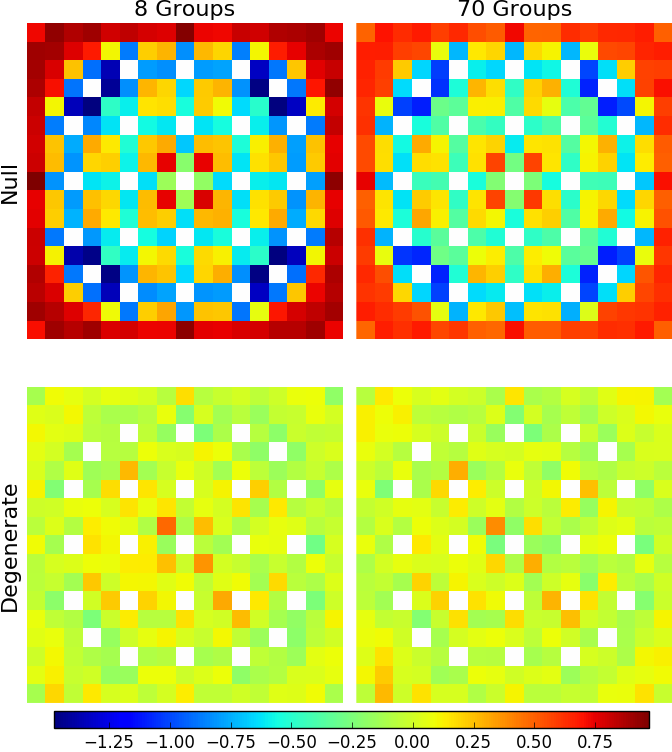
\includegraphics[width=\linewidth]{figures/quantification/assm-16/capt-err}
\caption[U-238 capture rate errors for a 1.6\% enriched assembly]{U-238 capture rate errors for a 1.6\% enriched assembly.}
\label{fig:chap8-assm-1.6-capt-err}
\end{figure}

\begin{figure}[h!]
\centering
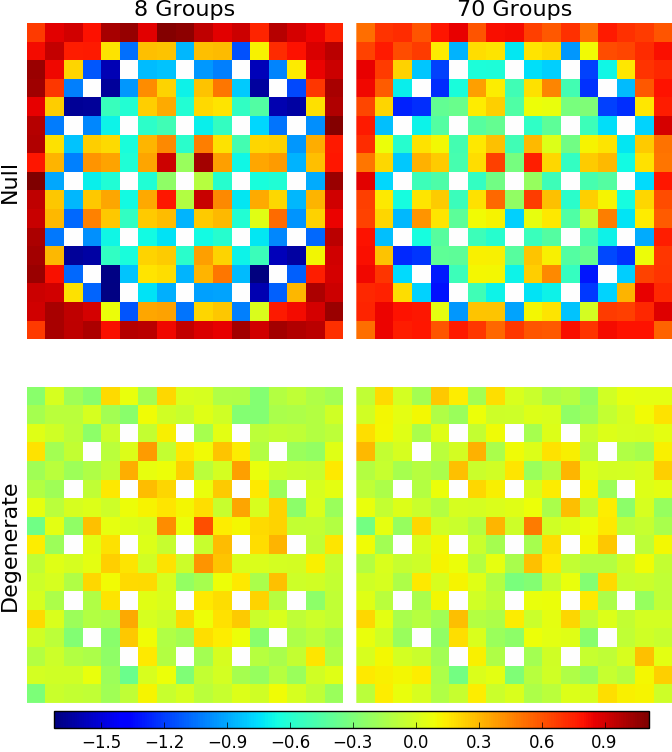
\includegraphics[width=\linewidth]{figures/quantification/assm-31/capt-err}
\caption[U-238 capture rate errors for a 3.1\% enriched assembly]{U-238 capture rate errors for a 3.1\% enriched assembly.}
\label{fig:chap8-assm-3.1-capt-err}
\end{figure}

\begin{figure}[h!]
\centering
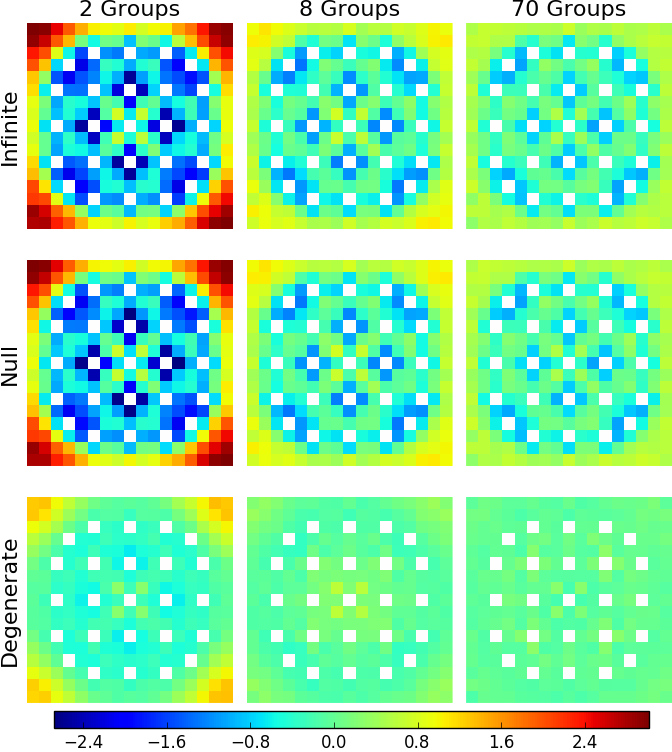
\includegraphics[width=\linewidth]{figures/quantification/assm-31-20BPs/capt-err}
\caption[U-238 capture rate errors for a 3.1\% enriched assembly with 20 BPs]{U-238 capture rate errors for a 3.1\% enriched assembly with 20 BPs.}
\label{fig:chap8-assm-3.1-20BPs-capt-err}
\end{figure}

\begin{figure}[h!]
\centering
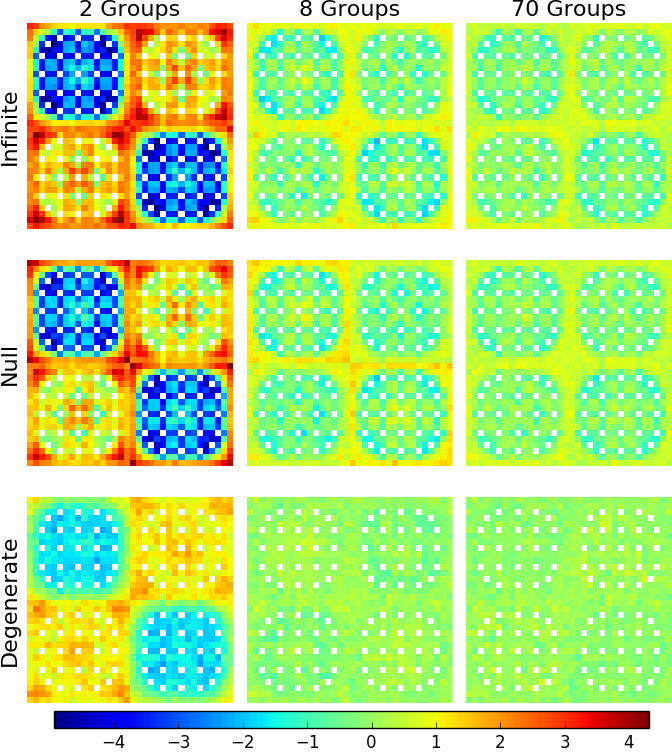
\includegraphics[width=\linewidth]{figures/quantification/2x2/capt-err}
\caption[U-238 capture rate errors for a 2$\times$2 colorset]{U-238 capture rate errors for a 2$\times$2 colorset.}
\label{fig:chap8-2x2-capt-err}
\end{figure}

\begin{figure}[h!]
\centering
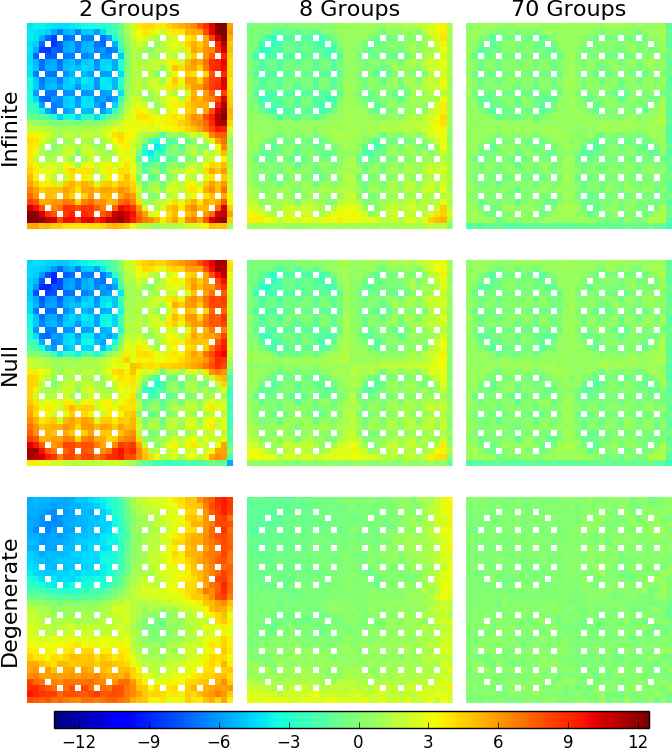
\includegraphics[width=\linewidth]{figures/quantification/reflector/capt-err}
\caption[U-238 capture rate errors for a 2$\times$2 colorset with a reflector]{U-238 capture rate errors for a 2$\times$2 colorset with a reflector.}
\label{fig:chap8-reflector-capt-err}
\end{figure}

\begin{figure}[h!]
\centering
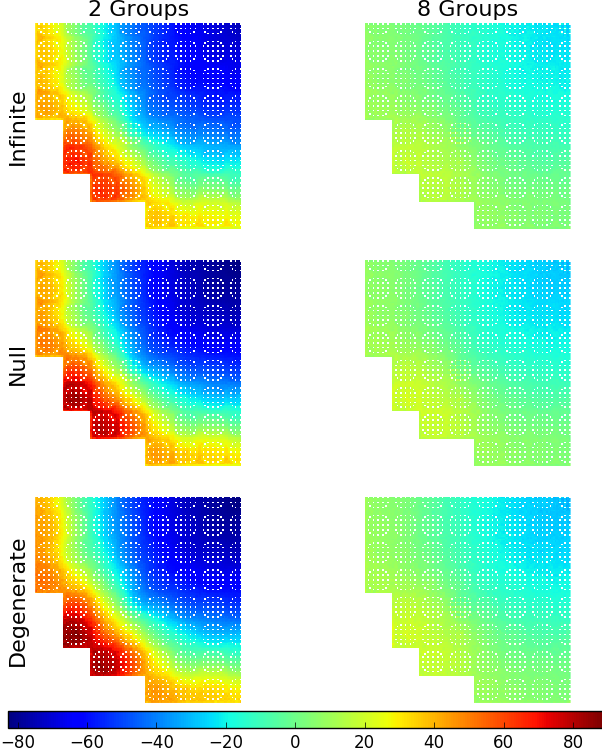
\includegraphics[width=\linewidth]{figures/quantification/full-core/capt-err}
\caption[U-238 capture rate errors for the 2D full core \ac{BEAVRS} model]{U-238 capture rate errors for the 2D full core \ac{BEAVRS} model.}
\label{fig:chap8-full-core-capt-err}
\end{figure}


\begin{itemize}[noitemsep]
  \item convergence rates for max/mean rel. err. for each benchmark
  \begin{itemize}[noitemsep]
    \item infinite vs. null vs. degenerate
    \item by energy group structure?
  \end{itemize}
  \item 2D heat maps of error distributions for each benchmark
  \begin{itemize}[noitemsep]
    \item infinite vs. null vs. degenerate
    \item by energy group structure?
  \end{itemize}
\end{itemize}


%%%%%%%%%%%%%%%%%%%%%%%%%%%%%%%%%%%%%%%%%%%%%%%%%%%%%%%%%%%%%%%%%%%%%%%%%%%%%%%
\section{MGXS Convergence Rates}
\label{sec:chap8-mgxs-converge}

\begin{itemize}[noitemsep]
  \item Plot evolution of rel. err. by batch for each homogenization scheme
  \begin{itemize}[noitemsep]
    \item groups with highest rel. err.
    \item reactions with greatest contribution to eigenvalue (U-238 capture)
    \item total (track-length) vs. scattering matrices (analog)    
    \item which group structure(s)?
 \end{itemize}
  \item compare to pin power convergence rates in preceding chapter
\end{itemize}

%-infinite vs. null vs. degenerate
%-conv rates for MGXS in each case - choose worst groups
%  -compare back to pin power error conv. rates
%  -convergence rates for infinite vs. null vs. degenerate